\documentclass[12pt,a4paper,oneside]{report}

% ---------------------------------------------------------------- layout (NITW guidelines: A4, Times New Roman
% 12 pt, 1.5 line spacing, left 30 mm, right 20 mm, header style with page number at the top right)
\usepackage[a4paper,left=30mm,right=20mm,top=15mm,bottom=22mm,headheight=15pt,headsep=12mm,footskip=10mm,
            includehead]{geometry}
\usepackage[T1]{fontenc}
\usepackage[utf8]{inputenc}
\usepackage{mathptmx}
\renewcommand{\ttdefault}{pcr}
\usepackage{setspace}
\onehalfspacing
\usepackage{graphicx}
\usepackage{booktabs}
\usepackage{tabularx}
\usepackage{xltabular}
\usepackage{array}
\usepackage{enumitem}
\usepackage{amsmath}
\usepackage[labelfont=bf,labelsep=space,font=small,justification=justified,singlelinecheck=true]{caption}
\captionsetup[table]{position=top,skip=4pt}
\usepackage{float}
\usepackage{tikz}
\usetikzlibrary{positioning,fit}
\usepackage{cite}
\usepackage{fancyhdr}
\usepackage{titletoc}
\usepackage{url}
\usepackage[colorlinks=true,linkcolor=blue,citecolor=blue,urlcolor=blue]{hyperref}
\urlstyle{same}
\setlength{\parskip}{3pt}
\renewcommand{\arraystretch}{1.15}
\newcolumntype{L}{>{\raggedright\arraybackslash}X}
\newcolumntype{P}[1]{>{\raggedright\arraybackslash}p{#1}}

\pagestyle{fancy}
\fancyhf{}
\makeatletter
\renewcommand{\chaptermark}[1]{\markboth{\@chapapp\ \thechapter.\ #1}{}}
\makeatother
\fancyhead[L]{\small\nouppercase{\leftmark}}
\fancyhead[R]{\small\thepage}
\renewcommand{\headrulewidth}{0.4pt}
\renewcommand{\footrulewidth}{0.4pt}
\fancypagestyle{plain}{\fancyhf{}\fancyfoot[C]{\small\thepage}\renewcommand{\headrulewidth}{0pt}%
  \renewcommand{\footrulewidth}{0.4pt}}
\renewcommand{\figurename}{Figure}

\newcommand{\projtitle}{SeizeLUT: A Self-Testing, Multiplier-Free Seizure Detector on an FPGA with Doctor Alerts}
\newcommand{\projtitleshort}{SeizeLUT: A Self-Testing, Multiplier-Free Seizure Detector on an FPGA}
\newcommand{\studentA}{Akshara Bonam}
\newcommand{\rollA}{23ECB0A11}
\newcommand{\studentB}{Sai Chaithr}
\newcommand{\rollB}{23ECB0A20}
\newcommand{\studentC}{Sowjanya}
\newcommand{\rollC}{23ECB0A22}
\newcommand{\students}{\studentA\ (\rollA), \studentB\ (\rollB) and \studentC\ (\rollC)}
\newcommand{\guide}{[Guide's name with title]}
\newcommand{\guidedesig}{[Designation]}
\newcommand{\dept}{Electronics and Communication Engineering}

\begin{document}

% ================================================================ title page
\begin{titlepage}
\centering
{\Large\bfseries SEIZELUT: A SELF-TESTING, MULTIPLIER-FREE SEIZURE DETECTOR ON AN FPGA WITH DOCTOR ALERTS\par}
\vspace{4mm}
{\large\bfseries From behind-the-ear EEG, ECG, EMG and motion to a seizure alarm in 1,202 FPGA lookup tables\par}
\vspace{12mm}
{\itshape\bfseries BISP Project Report submitted to the\\
National Institute of Technology Warangal\\
as part of the requirements for the degree\par}
\vspace{5mm}
{\itshape\bfseries of\par}
\vspace{5mm}
{\large\bfseries Bachelor of Technology\\ in \dept\par}
\vspace{5mm}
{\itshape\bfseries by\par}
\vspace{4mm}
{\large\bfseries \studentA} (Roll No. \rollA)\par
{\large\bfseries \studentB} (Roll No. \rollB)\par
{\large\bfseries \studentC} (Roll No. \rollC)\par
\vspace{8mm}
Under the guidance of\par
\vspace{3mm}
{\large\bfseries \guide\par}
{\small \guidedesig, Department of \dept\par}
\vspace{8mm}

\includegraphics[width=28mm]{figures/nitw_logo.png}\par
\vfill
{\bfseries DEPARTMENT OF ELECTRONICS AND COMMUNICATION ENGINEERING\\[1mm]
NATIONAL INSTITUTE OF TECHNOLOGY WARANGAL\\[1mm]
November 2026\par}
\end{titlepage}

\pagenumbering{roman}
\setcounter{page}{2}

% ================================================================ approval
\chapter*{\centering\normalsize\bfseries\large APPROVAL OF THE PROJECT EVALUATION BOARD}
\addcontentsline{toc}{chapter}{Certificate of Approval}
\thispagestyle{plain}
\hfill DD/MM/YYYY

\vspace{8mm}
Certified that the report entitled \textbf{\projtitle} submitted by \students\ to the National Institute of
Technology Warangal, as the BISP project report of the Bachelor of Technology programme in \dept, has been examined
and accepted by the evaluation board.

\vspace{30mm}
\noindent(Member of the Board)\hfill(Member of the Board)\hfill(Member of the Board)

\vspace{30mm}
\noindent(Supervisor)\hfill(Co-Supervisor)

\vspace{30mm}
\noindent(Head of the Department)\hfill(Chairperson, Evaluation Board)

% ================================================================ certificate
\chapter*{}
\addcontentsline{toc}{chapter}{Certificate}
\thispagestyle{plain}
\vspace{-30mm}
\begin{center}
(The certificate is to be printed on the Departmental Letter-Head)\\[14mm]
{\large\bfseries\underline{CERTIFICATE}}
\end{center}
\vspace{8mm}
This is to certify that the report entitled \textbf{\projtitle}, submitted by \textbf{\students} to the
National Institute of Technology Warangal, is a record of bona fide project work carried out by the students under
my (our) supervision as the BISP project of the Bachelor of Technology programme in \dept.

\vspace{40mm}
\noindent\rule{60mm}{0.4pt}\\
\hspace*{14mm}Supervisor\\
\hspace*{4mm}\guide

\vspace{15mm}
\noindent Date:

% ================================================================ declaration
\chapter*{\centering\large\bfseries DECLARATION}
\addcontentsline{toc}{chapter}{Declaration}
\thispagestyle{plain}
We certify that
\begin{enumerate}[label=\alph*.]
\item The work contained in the report is original and has been done by us under the general supervision of our
  supervisor(s).
\item The work has not been submitted to any other Institute for any degree or diploma.
\item We have followed the guidelines provided by the Institute in writing the report.
\item Whenever we have used materials (data, theoretical analysis, and text) from other sources, we have given due
  credit to them by citing them in the text of the report and giving their details in the references.
\item Whenever we have quoted written materials from other sources, we have put them under quotation marks and given
  due credit to the sources by citing them and giving required details in the references.
\item An AI assistant was used to help write analysis code, check results and draft parts of the text. All numbers
  in this report come from our saved experiment records, scripts and board measurements, and we take
  responsibility for the content.
\end{enumerate}

\vspace{25mm}
\noindent
\begin{tabular}{@{}c@{}}\rule{42mm}{0.4pt}\\ \studentA\\ (\rollA)\end{tabular}\hfill
\begin{tabular}{@{}c@{}}\rule{42mm}{0.4pt}\\ \studentB\\ (\rollB)\end{tabular}\hfill
\begin{tabular}{@{}c@{}}\rule{42mm}{0.4pt}\\ \studentC\\ (\rollC)\end{tabular}

% ================================================================ acknowledgements
\chapter*{Acknowledgements}
\addcontentsline{toc}{chapter}{Acknowledgements}
\thispagestyle{plain}
We thank our project guide, \guide, \guidedesig, Department of \dept, for the guidance and encouragement given
throughout this project.

We thank the Head of the Department and the faculty of the Department of \dept, National Institute of Technology
Warangal, for the facilities and support provided. We also thank the SeizeIT2 consortium for releasing the dataset
used in this work publicly, and the authors of the open-source tools on which our software builds.

Finally, we thank our families and friends for their support.

\vspace{10mm}
\hfill\textbf{\studentA, \studentB, \studentC}

% ================================================================ abstract
\chapter*{Abstract}
\addcontentsline{toc}{chapter}{Abstract}
\markboth{Abstract}{}

Epileptic seizures are often missed by patients and carers, and a wearable detector must run for days on a small
battery while it can be trusted to compute what was validated. We built SeizeLUT, a seizure detector whose classifier
is a Differentiable Weightless Neural Network (DWN) of 50 six-input lookup tables (LUTs) that map one-to-one onto
FPGA LUTs, fed by a bit-exact integer front end for behind-the-ear EEG, ECG, EMG and motion that needs no multiplier.

On the official split of the SeizeIT2 dataset (125 patients, 11,626 hours), every design choice was made by
cross-validation on the 96 training patients, and the frozen detector was scored once on the 29 held-out test
patients: event-F1 $0.248 \pm 0.016$ with 0.8 false alarms per day, above a TreeLUT model, a logic-gate network, an
INT8 network and the ChronoNet baseline, in 398 FPGA LUTs with no DSP block. A two-stage version that confirms each
alarm against the post-ictal period detects 73.3\,\% of seizures at 10.9 false alarms per hour, against 71.1\,\% at
11.0 for the dataset paper's SVM.

Because the classifier is a set of truth tables, every single hardware fault (3,592 of them) can be enumerated and
judged by its clinical effect on 8,714 hours of training data. 255 test vectors chosen for coverage detect every
fault that changes a decision, and the on-chip self-test runs them in 10.3\,\textmu s. A microcoded shift-add engine
computes the features in the FPGA fabric, so the whole detector, front end included, is multiplier-free hardware of
1,202 LUTs that keeps up with the sensors at under 1\,MHz.

The complete system runs on an AMD Kria KV260 board. All nine board tests pass: the self-test, the replay of 431,960
one-second windows with no mismatch, all 3,592 injected faults detected exactly as predicted, and raw signals through
the front end and classifier in the fabric with every feature and decision equal to the software. A live demo drives
an alarm LED and a buzzer, and an ESP32 sends the doctor a push notification with the measured heart rate, movement,
muscle and brain activity, an action to take, and escalation after 2 and 5 minutes.


% ================================================================ lists
\cleardoublepage
\phantomsection
\addcontentsline{toc}{chapter}{Contents}
\tableofcontents
\cleardoublepage
\phantomsection
\addcontentsline{toc}{chapter}{List of Figures}
\listoffigures
\cleardoublepage
\phantomsection
\addcontentsline{toc}{chapter}{List of Tables}
\listoftables
\chapter*{List of Abbreviations}
\addcontentsline{toc}{chapter}{List of Abbreviations}
\markboth{List of Abbreviations}{}
\begin{longtable}{@{}p{30mm}p{120mm}@{}}
ACC & Accelerometer\\
ASIC & Application-specific integrated circuit\\
AUPR & Area under the precision--recall curve\\
AUROC & Area under the receiver operating characteristic curve\\
bte-EEG & Behind-the-ear electroencephalography\\
CNN & Convolutional neural network\\
CV & Cross-validation\\
DSP & Digital signal processing block (FPGA multiplier)\\
DWN & Differentiable Weightless Neural Network\\
ECG & Electrocardiography\\
EDF & European Data Format\\
EFD & Extended Finite Difference\\
EMG & Electromyography\\
FA & Focal aware (seizure); false alarm\\
FBTC & Focal to bilateral tonic-clonic (seizure)\\
FIA & Focal impaired awareness (seizure)\\
FP/24 h & False positives (false alarms) per 24 hours\\
FPGA & Field-programmable gate array\\
GBDT & Gradient-boosted decision trees\\
GRU & Gated recurrent unit\\
GYR & Gyroscope\\
iEEG & Intracranial EEG\\
ILAE & International League Against Epilepsy\\
INT8 & 8-bit integer format\\
LGN & Logic-gate network\\
LSB & Least significant bit\\
LUT & Lookup table (LUT6: six-input lookup table)\\
MCU & Microcontroller\\
MI & Mutual information\\
MIL & Multiple-instance learning\\
MLP & Multilayer perceptron\\
OVLP & Any-overlap event scoring\\
SoC & System on chip\\
SUDEP & Sudden unexpected death in epilepsy\\
SVM & Support vector machine\\
SzCORE & Seizure Community Open-Source Research Evaluation framework\\
TCN & Temporal convolutional network\\
TUSZ & Temple University Hospital Seizure Corpus\\
WNN & Weightless neural network\\
AXI & Advanced eXtensible Interface (on-chip bus)\\
BIST & Built-in self-test\\
ESP32 & Low-cost microcontroller with Wi-Fi (Espressif)\\
KV260 & AMD Kria KV260 Vision AI Starter Kit (FPGA board)\\
PMOD & Peripheral module connector of the board\\
PYNQ & Python productivity for Zynq (board software framework)\\
SOM & System-on-module (the K26 on the KV260)\\
\end{longtable}


% ================================================================ chapters
\cleardoublepage
\pagenumbering{arabic}
\chapter{Introduction}\label{ch:intro}

\section{Motivation}

\begin{itemize}
\item Epilepsy affected an estimated 45.9 million people in 2016 \cite{gbd2019epilepsy}. Patients often miss their own
  seizures, so diaries undercount them \cite{elger2018underreporting}, and tonic-clonic seizures carry a risk of sudden
  death \cite{ryvlin2013mortemus}.
\item Wearables are recommended today only for tonic-clonic seizures \cite{beniczky2021guideline}; for focal seizures
  (822 of the 883 in SeizeIT2) false alarms are the main obstacle \cite{swinnen2026seizeit2}.
\item Behind-the-ear EEG with ECG, EMG and motion is a discreet alternative \cite{vandecasteele2020bte,vandecasteele2021ecg};
  SeizeIT2 \cite{bhagubai2025seizeit2} provides 125 patients recorded with such a wearable.
\item A wearable detector must run for days on a small battery. Multiplications dominate the cost of neural networks
  in hardware, while an FPGA's basic element is a 6-input lookup table (LUT). \emph{LUT-native} networks
  \cite{bacellar2024dwn,petersen2022dlgn,umuroglu2020logicnets} are built from exactly this element.
\item A medical device must also not fail silently: a hardware fault in the classifier turns into missed seizures or
  false alarms, and an alarm is only useful if the right person can act on it quickly.
\end{itemize}

\section{Problem Statement and Objectives}

\begin{quote}
\itshape Can a LUT-native network, fed by integer features from behind-the-ear EEG, ECG, EMG and motion, detect
seizures in unseen patients as well as the published SeizeIT2 baselines, as multiplier-free hardware that can test
itself, run on a real FPGA board, and alert a doctor?
\end{quote}

\begin{table}[H]
\centering\small
\caption{Objectives and their status.}\label{tab:objectives}
\begin{tabularx}{\textwidth}{@{}cLP{42mm}@{}}
\toprule
\textbf{\#} & \textbf{Objective} & \textbf{Status}\\
\midrule
1 & Audit SeizeIT2 and reproduce its published baselines & Done\\
2 & Integer-only, bit-exact multimodal feature pipeline & Done\\
3 & Compare LUT-native, tree and multiplier-based models on accuracy and hardware cost & Done\\
4 & Extend the LUT network for wearables (distillation, missing sensors, post-ictal verification) & Done\\
5 & Evaluate the frozen design once on the 29 held-out test patients & Done\\
6 & Self-testing: complete single-fault analysis and an on-chip test that detects every relevant fault & Done, measured on the board\\
7 & Front end and classifier in the FPGA fabric; KV260 implementation & Done, all 9 board tests pass\\
8 & Live demo with alarm LED and buzzer & Done on the board\\
9 & Doctor alert through an ESP32 (phone notification and live page) & Built and tested in emulation; ESP32 hardware test pending\\
\bottomrule
\end{tabularx}
\end{table}

\section{Contributions}

\begin{itemize}
\item The first LUT-native seizure detector, and the first benchmark of LUT-family models (DWN, logic-gate network,
  TreeLUT) against standard machine learning on SeizeIT2 with event-level clinical scoring.
\item A bit-exact, multiplier-free integer front end, and a microcoded engine that computes it in the FPGA fabric:
  the whole detector is 1,202 LUTs with no multiplier.
\item Distillation from a tree ensemble into the LUT network (false alarms per day from 2.4 to 0.9) and a LUT-native
  post-ictal verification stage that detects more seizures than the dataset paper's SVM.
\item \emph{Self-testing}: every one of the 3,592 single faults of the classifier judged by its effect on decisions,
  and 255 selected test vectors that detect all decision-relevant faults; verified fault by fault on the board.
\item A complete Kria KV260 implementation with a nine-step board test campaign, a live demo, and a doctor alert
  that tells the doctor what to do.
\item An independent reproduction of the SeizeIT2 ChronoNet baseline, including a protocol with no test information.
\end{itemize}

\section{Team}

\begin{table}[H]
\centering\small
\caption{Project team.}\label{tab:team}
\begin{tabular}{@{}ll@{}}
\toprule
\textbf{Name} & \textbf{Roll number}\\
\midrule
\studentA & \rollA\\
\studentB & \rollB\\
\studentC & \rollC\\
\bottomrule
\end{tabular}
\end{table}

\section{Organisation of the Report}

Chapter~\ref{ch:lit} reviews the literature, Chapter~\ref{ch:method} the dataset and method, Chapter~\ref{ch:results}
the detection results, Chapter~\ref{ch:hw} the FPGA hardware, self-test and board results, Chapter~\ref{ch:alert} the
doctor alert, Chapter~\ref{ch:challenges} the challenges, and Chapter~\ref{ch:concl} the conclusions, the publication
plan and future work.

\chapter{Literature Review}\label{ch:lit}

The survey covers 79 references in four areas. Each was checked against its published record; numbers are as reported
in the cited abstracts.

\section{Epilepsy and Wearable Seizure Detection}\label{sec:lit-clinical}\label{sec:lit-wearable}

\begin{itemize}
\item \textbf{Clinical need.} Seizures are classified by onset and awareness \cite{fisher2017ilae}; unaware patients
  under-report them \cite{elger2018underreporting}; the ILAE--IFCN guideline recommends wearables only for tonic-clonic
  seizures \cite{beniczky2021guideline}.
\item \textbf{Devices.} EMG, wristband and multimodal devices detect convulsive seizures well
  \cite{leijten2018review,beniczky2018emg,onorati2017empatica,regalia2019empatica,naganur2022meta}; focal seizures
  remain open.
\item \textbf{Behind-the-ear EEG (SeizeIT).} Two behind-the-ear channels detect seizures \cite{vandecasteele2020bte};
  ECG adds 8--11\,\% sensitivity \cite{vandecasteele2021ecg,bhagubai2023ecg}; tree ensembles won the 2023 challenge
  \cite{bhagubai2024challenge}; SeizeIT2 released 125 patients \cite{bhagubai2025seizeit2}; a 192-adult validation
  reached precision 0.004 before review \cite{swinnen2026seizeit2}; ECG-only \cite{reintjes2025ecg} and complex-valued
  multimodal \cite{su2026cmepinet} detectors also use SeizeIT2.
\item \textbf{Fusion.} Adding EMG and motion mainly removes false alarms \cite{zhang2024tcs}; only one work handles a
  missing modality \cite{zhang2024cyclic}.
\end{itemize}

\begin{table}[htbp]
\centering\small
\caption{Wearable and multimodal seizure detection studies (results as reported).}\label{tab:lit-wearable}
\begin{tabularx}{\textwidth}{@{}P{30mm}cP{22mm}P{22mm}LL@{}}
\toprule
\textbf{Work} & \textbf{Year} & \textbf{Signals} & \textbf{Seizures} & \textbf{Result} & \textbf{Gap for our problem}\\
\midrule
Beniczky et al. \cite{beniczky2018emg} & 2018 & EMG & tonic-clonic & $>$90\,\% sensitivity & convulsive only\\
Onorati et al. \cite{onorati2017empatica} & 2017 & EDA + ACC & convulsive & 94.55\,\%, 0.2 FA/day & convulsive only\\
Naganur et al. \cite{naganur2022meta} & 2022 & meta-analysis & tonic-clonic & 0.91, 2.1 FA/24\,h & focal not solved\\
Vandecasteele et al. \cite{vandecasteele2020bte} & 2020 & bte-EEG & focal & 64.1\,\%, 2.8 FP/24\,h (patient-independent) & EEG only\\
Vandecasteele et al. \cite{vandecasteele2021ecg} & 2021 & bte-EEG + ECG & focal & +8--11\,\% sensitivity with ECG & software only\\
Bhagubai et al. \cite{bhagubai2024challenge} & 2024 & bte-EEG & challenge & tree ensemble won & no hardware budget\\
Zhang et al. \cite{zhang2024tcs} & 2024 & EEG + EMG + ACC & tonic-clonic & 90.9\,\%, 0.1 FP/24\,h & tonic-clonic only\\
Swinnen et al. \cite{swinnen2026seizeit2} & 2026 & SeizeIT2 wearable & focal, 192 adults & 0.73 at precision 0.004 & false alarms\\
BrainFuseNet \cite{ingolfsson2024brainfusenet} & 2024 & EEG + PPG + ACC & -- & 64.28\,\%, 0.21 FP/h, MCU & multipliers, no ECG/EMG\\
Zhang et al. \cite{zhang2024cyclic} & 2024 & EEG + EMG & -- & -- & large transformer\\
\bottomrule
\end{tabularx}
\end{table}

\section{Detection Algorithms and Evaluation}\label{sec:lit-alg}

\begin{itemize}
\item \textbf{Feature-based models} work well but are often patient-specific \cite{shoeb2010icml}; tree ensembles are
  strongest on SeizeIT data \cite{alhussaini2023seizft,huang2023lightweight}.
\item \textbf{Deep models} (ChronoNet \cite{roy2019chrononet}, EEGNet \cite{lawhern2018eegnet}, EEGWaveNet
  \cite{thuwajit2022eegwavenet}, graph and transformer models \cite{tang2022gnnssl,wu2025seizuretransformer,yang2023biot})
  are large and multiplier-based; ChronoNet trained on SeizeIT1 reached 15.2\,\% sensitivity on SeizeIT2
  \cite{huang2023lightweight}.
\item \textbf{Imperfect labels}: weak supervision, MIL, noisy-label training and distillation
  \cite{saab2020weak,isaev2020mil,shama2026bundl,zheng2023kdgnn} motivate our extensions N4 and N5.
\item \textbf{Evaluation} varies between papers and corpora \cite{ziyabari2017metrics,shah2018tusz}; SzCORE standardises event metrics
  \cite{dan2024szcore}; in a blind benchmark the best event-F1 was 43\,\% \cite{dan2025szcorechallenge}; subject leakage
  inflates results \cite{brookshire2024leakage}.
\end{itemize}

\begin{table}[htbp]
\centering\small
\caption{Seizure detection algorithms and evaluation frameworks (results as reported).}\label{tab:lit-alg}
\begin{tabularx}{\textwidth}{@{}P{30mm}cP{25mm}P{20mm}LL@{}}
\toprule
\textbf{Work} & \textbf{Year} & \textbf{Method} & \textbf{Data} & \textbf{Result} & \textbf{Gap for our problem}\\
\midrule
Shoeb \& Guttag \cite{shoeb2010icml} & 2010 & patient-specific SVM & CHB-MIT & 96\,\% of seizures, 2 FD/24\,h & patient-specific, scalp\\
SeizFt \cite{alhussaini2023seizft} & 2023 & features + CatBoost & SeizeIT1/2 & ICASSP 2023 winner & EEG only, no hardware cost\\
Huang et al. \cite{huang2023lightweight} & 2023 & random forest; ChronoNet & SeizeIT1/2 & RF 73.6\,\%; ChronoNet 15.2\,\% & EEG only\\
ChronoNet \cite{roy2019chrononet} & 2019 & CNN + GRU & TUH abnormal & benchmark at the time & large, multipliers\\
EEGWaveNet \cite{thuwajit2022eegwavenet} & 2022 & multiscale CNN & CHB-MIT, TUSZ & better subject-independent & scalp, float CNN\\
Tang et al. \cite{tang2022gnnssl} & 2022 & self-supervised GNN & TUSZ & AUROC 0.875 & needs full montage\\
Shama \& Venkataraman \cite{shama2026bundl} & 2026 & noisy-label training & TUH, CHB-MIT & robust to label noise & scalp EEG\\
Zheng et al. \cite{zheng2023kdgnn} & 2023 & distilled GNN & TUSZ & competitive with 2 channels & float student\\
SzCORE \cite{dan2024szcore} & 2024 & evaluation framework & scalp EEG & standard event metrics & not for wearables\\
SzCORE challenge \cite{dan2025szcorechallenge} & 2025 & blind benchmark & 65 subjects & best event-F1 43\,\% & scalp EEG\\
\bottomrule
\end{tabularx}
\end{table}

\section{LUT-Native, Weightless and Logic Networks}\label{sec:lit-lut}

\begin{itemize}
\item \textbf{Weightless networks} replace weighted sums with memory lookups \cite{aleksander1984wisard,susskind2022bthowen,susskind2023uleen};
  the \textbf{DWN} made LUT contents and input mapping trainable by gradient descent \cite{bacellar2024dwn}, later applied to
  activity recognition and control \cite{bacellar2025nanoml,kresse2025dwc}.
\item \textbf{Logic-gate networks} learn 2-input gates \cite{petersen2022dlgn,petersen2024convdlgn,ruttgers2026lightdlgn};
  a recurrent version exists for language \cite{buhrer2025rdlgn}.
\item \textbf{LUT networks for FPGAs}: LUTNet, LogicNets, PolyLUT, NeuraLUT, AmigoLUT, ReducedLUT and TreeLUT
  \cite{wang2019lutnet,umuroglu2020logicnets,andronic2023polylut,andronic2024neuralut,weng2025amigolut,cassidy2025reducedlut,khataei2025treelut}.
\item \textbf{The encoder} can dominate the cost of small DWNs \cite{mecik2025thermo}; in our final network it is 776 of
  895 LUTs.
\item \textbf{Biosignals}: ECG \cite{mommen2026ecg} and EEG classification \cite{dharia2026eeglgn}; the only weightless
  seizure work is a 4-patient study \cite{deaguiar2015wisard}.
\end{itemize}

\begin{table}[htbp]
\centering\small
\caption{LUT-native, weightless and logic networks (results as reported).}\label{tab:lit-lut}
\begin{tabularx}{\textwidth}{@{}P{30mm}cP{27mm}P{22mm}LL@{}}
\toprule
\textbf{Work} & \textbf{Year} & \textbf{Model} & \textbf{Domain} & \textbf{Hardware / result} & \textbf{Gap}\\
\midrule
WiSARD \cite{aleksander1984wisard} & 1984 & RAM-node WNN & images & -- & no gradient training\\
ULEEN \cite{susskind2023uleen} & 2023 & weightless & MLPerf Tiny & 7.1$\times$ energy eff.\ vs FINN & no biosignals\\
DWN \cite{bacellar2024dwn} & 2024 & differentiable LUT6 net & tabular & FPGA, MCU & stateless, no events\\
nanoML HAR \cite{bacellar2025nanoml} & 2025 & DWN & inertial HAR & 56--104\,nJ / sample & single modality\\
LGN \cite{petersen2022dlgn} & 2022 & 2-input logic gates & images & $>$1\,M images/s (CPU) & no biosignals\\
Recurrent LGN \cite{buhrer2025rdlgn} & 2025 & stateful logic gates & translation & -- & no hardware\\
LogicNets \cite{umuroglu2020logicnets} & 2020 & sparse quantised LUT net & jet tagging & $<$15\,ns latency & tiny fan-in\\
NeuraLUT \cite{andronic2024neuralut} & 2024 & dense sub-nets in LUTs & jet tagging & 4.3$\times$ lower latency & static\\
TreeLUT \cite{khataei2025treelut} & 2025 & quantised GBDT & tabular & 4--101$\times$ lower area-delay & per window\\
Mecik \& Kumm \cite{mecik2025thermo} & 2025 & DWN generator & jet tagging & encoder up to 3.2$\times$ LUTs & --\\
Mommen et al. \cite{mommen2026ecg} & 2026 & LGN, LUT network & ECG arrhythmia & 2.0--3.0k LUTs, 5--7\,mW & single modality\\
Dharia et al. \cite{dharia2026eeglgn} & 2026 & LGN & EEG & embedded CPU & no FPGA, no seizures\\
de Aguiar et al. \cite{deaguiar2015wisard} & 2015 & WiSARD & seizure anticipation & -- & 4 patients, accuracy only\\
\bottomrule
\end{tabularx}
\end{table}

\section{Hardware Seizure Detectors}\label{sec:lit-hw}

\begin{itemize}
\item \textbf{ASICs} reach nJ--\textmu J per decision with SVMs and trees
  \cite{verma2010micro,altaf2015jssc,altaf2016tbcas,huang2020jssc,shoaran2018jetcas,shin2022neuraltree}.
\item \textbf{FPGAs}: SVM, line-length and spiking-network detectors
  \cite{wang2018access,elhosary2019tbcas,razi2022tbcas,vittimberga2025sensors,busia2025fpga}; the closest to ours is an SNN
  on a small iCE40 \cite{busia2025fpga}.
\item \textbf{Microcontrollers}: e-Glass, EEGformer, BrainFuseNet \cite{sopic2018eglass,busia2024eegformer,ingolfsson2024brainfusenet} and low-power EEG platforms \cite{kartsch2019biowolf,ingolfsson2022artifact};
  efficient-inference tools: BNNs, FINN, INT8 quantisation, hls4ml
  \cite{hubara2016bnn,umuroglu2017finn,jacob2018quant,duarte2018hls4ml}.
\item Nearly all use EEG only, per-patient training and epoch-level metrics; none maps the classifier into LUTs.
\end{itemize}

\begin{table}[htbp]
\centering\footnotesize
\caption{Hardware seizure detectors (results as reported; units differ between papers).}\label{tab:lit-hw}
\begin{tabularx}{\textwidth}{@{}P{25mm}@{\hspace{4pt}}c@{\hspace{4pt}}P{17mm}P{16mm}P{22mm}LL@{}}
\toprule
\textbf{Work} & \textbf{Year} & \textbf{Platform} & \textbf{Signals} & \textbf{Hardware} & \textbf{Detection} & \textbf{Gap}\\
\midrule
Verma et al. \cite{verma2010micro} & 2010 & ASIC & scalp EEG & 9\,\textmu J / feature vector & classifier off-chip & EEG only\\
Bin Altaf et al. \cite{altaf2015jssc} & 2015 & ASIC & scalp EEG & 2.73\,\textmu J / class. & 95.7\,\% (epoch) & per patient\\
Shoaran et al. \cite{shoaran2018jetcas} & 2018 & ASIC & iEEG & 41.2\,nJ / class. & F1 87.9\,\% & implant\\
NeuralTree \cite{shin2022neuraltree} & 2022 & ASIC & EEG, iEEG & 0.227\,\textmu J / class. & 95.6\,\% (EEG) & neural only\\
Wang et al. \cite{wang2018access} & 2018 & FPGA (Zynq) & scalp EEG & 380\,mW & 98.4\,\%, 0.356 FD/h & per patient\\
Farhang Razi \& Schmid \cite{razi2022tbcas} & 2022 & FPGA (Cyclone V) & iEEG & 0.49\,mW dynamic & 100\,\% sens. & implant\\
Busia et al. \cite{busia2025fpga} & 2025 & FPGA (iCE40) & scalp EEG & 4.55\,nJ / inference & 0.3 FP/h & EEG only\\
e-Glass \cite{sopic2018eglass} & 2018 & MCU & scalp EEG & 2.71 days / charge & 93.8\,\% (epoch) & EEG only\\
EEGformer \cite{busia2024eegformer} & 2024 & MCU & scalp EEG & 0.31\,mJ / inference & 73\,\%, 0.15 FP/h & multipliers\\
BrainFuseNet \cite{ingolfsson2024brainfusenet} & 2024 & MCU & EEG, PPG, ACC & 0.11\,mJ / inference & 0.21 FP/h & no ECG/EMG\\
\bottomrule
\end{tabularx}
\end{table}

\clearpage
\section{Research Gaps}\label{sec:lit-gaps}

\begin{xltabular}{\textwidth}{@{}cP{45mm}LL@{}}
\caption{Research gaps and how this project addresses them.}\label{tab:lit-gaps}\\
\toprule
\textbf{\#} & \textbf{Gap} & \textbf{Evidence} & \textbf{How this project addresses it}\\
\midrule
\endfirsthead
\toprule
\textbf{\#} & \textbf{Gap} & \textbf{Evidence} & \textbf{How this project addresses it}\\
\midrule
\endhead
\small 1 & \small No LUT-native (weightless, logic-gate or LUT) seizure detector exists & \small LUT networks are benchmarked on images, physics and tabular data; the only weightless seizure work is a 4-patient study \cite{deaguiar2015wisard} & \small First benchmark of DWN, LGN, TreeLUT and LogicNets-style networks for seizure detection, on SeizeIT2\\
\small 2 & \small Hardware detectors use EEG alone, although fusion is the most consistent way to cut false alarms & \small \cite{vandecasteele2021ecg,zhang2024tcs}; Section~\ref{sec:lit-hw} & \small Integer features from behind-the-ear EEG, ECG, EMG and motion in one bit-exact front end\\
\small 3 & \small Missing sensors are rarely handled; LUT networks never & \small \cite{zhang2024cyclic}; Section~\ref{sec:lit-lut} & \small Presence bits, modality dropout, gated and late fusion, missing-sensor tests (N6)\\
\small 4 & \small The encoder's hardware cost is ignored, although it dominates small LUT networks & \small \cite{mecik2025thermo}; our estimate: about 850 of 960 LUTs & \small Cost model that counts every comparator; comparator-budgeted and learned encoders (N2)\\
\small 5 & \small LUT networks are stateless; seizures unfold over tens of seconds & \small \cite{buhrer2025rdlgn} & \small A stateful DWN with state bits fed back every second (N1)\\
\small 6 & \small Results are patient-specific, leak between training and test, or use incomparable metrics & \small \cite{brookshire2024leakage,ziyabari2017metrics,dan2025szcorechallenge} & \small Patient-wise cross-validation, a locked test set used once, SzCORE metrics with the paper's metrics alongside\\
\small 7 & \small Small models learn from noisy labels and from larger models only in floating point & \small \cite{shama2026bundl,zheng2023kdgnn} & \small Noise-robust and multiple-instance losses (N5) and distillation from LightGBM (N4) into a LUT network\\
\small 8 & \small Detectors are black boxes & \small Section~\ref{sec:lit-lut} & \small Tracing alarms to the inputs read by each LUT (N7)\\
\small 9 & \small Published wearable baselines are not independently reproduced & \small Section~\ref{sec:lit-wearable} & \small Independent reproduction of the SeizeIT2 ChronoNet baseline, with and without test-patient information\\
\bottomrule
\end{xltabular}

\chapter{Dataset, Methodology and Experimental Setup}\label{ch:method}

\section{SeizeIT2 Dataset}

SeizeIT2 \cite{bhagubai2025seizeit2} (OpenNeuro ds005873 v1.1.0, CC0) holds wearable recordings of 125 patients with
focal epilepsy from five European epilepsy units, with seizures annotated on hospital video-EEG. We use the official
split: \textbf{96 training patients} for all development and \textbf{29 test patients} scored once, after the design
was frozen. Tables~\ref{tab:modalities} and~\ref{tab:inventory} and Figures~\ref{fig:classes} and~\ref{fig:hours}
summarise it (all values measured by our audit).

\begin{table}[H]
\centering\small
\caption{Signals recorded by the wearable (rates measured from the files).}\label{tab:modalities}
\begin{tabular}{@{}llc@{}}
\toprule
\textbf{Signal} & \textbf{Channels} & \textbf{Rate}\\
\midrule
Behind-the-ear EEG & 2 (left, right or cross-head) & 256 Hz\\
ECG & 1 & 256 Hz\\
EMG & 1 & 256 Hz\\
Motion & 3-axis accelerometer + 3-axis gyroscope & 25 Hz\\
\bottomrule
\end{tabular}
\end{table}

\begin{table}[H]
\centering\small
\caption{Inventory of SeizeIT2 measured by our audit.}\label{tab:inventory}
\begin{tabular}{@{}ll@{}}
\toprule
\textbf{Quantity} & \textbf{Value}\\
\midrule
Patients / recordings / EDF files & 125 / 2,850 / 11,009 (125.9 GB)\\
Hours of EEG & 11,626 h (median 95 h per patient)\\
Seizures & 883 (train 702, test 181)\\
Seizure time & 14.3 h = \textbf{0.123\,\%} of the recording time\\
Seizure duration & 2--962 s (median 33 s)\\
Missing ECG/EMG; missing motion & 3.1\,\%; 3.9\,\% of the time\\
\bottomrule
\end{tabular}
\end{table}

\begin{figure}[H]
\centering
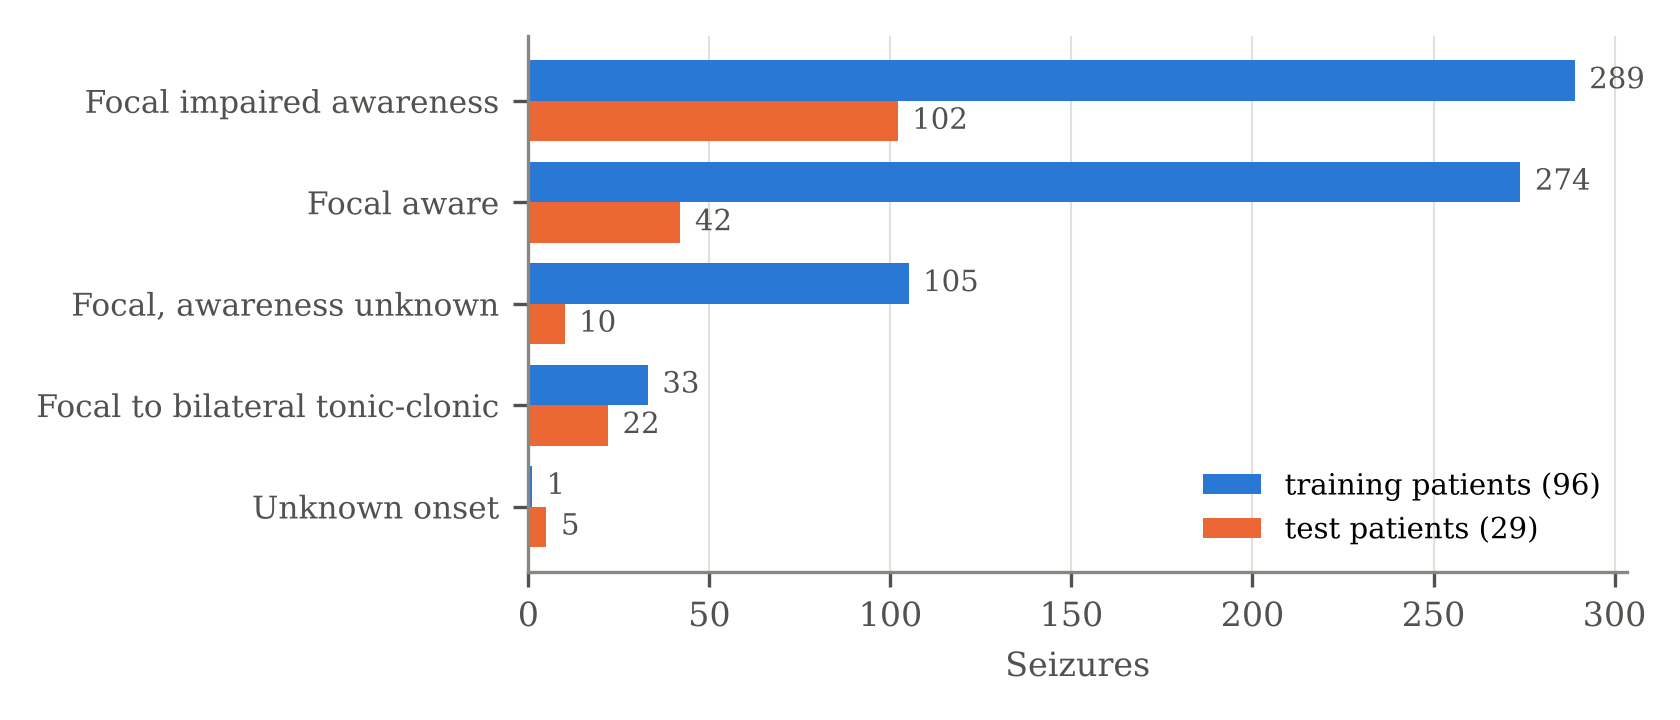
\includegraphics[width=0.78\textwidth]{figures/seizure_classes.png}
\caption{Seizure classes in the training and test patients: 822 of 883 seizures are focal seizures that do not become
tonic-clonic.}\label{fig:classes}
\end{figure}

\begin{figure}[H]
\centering
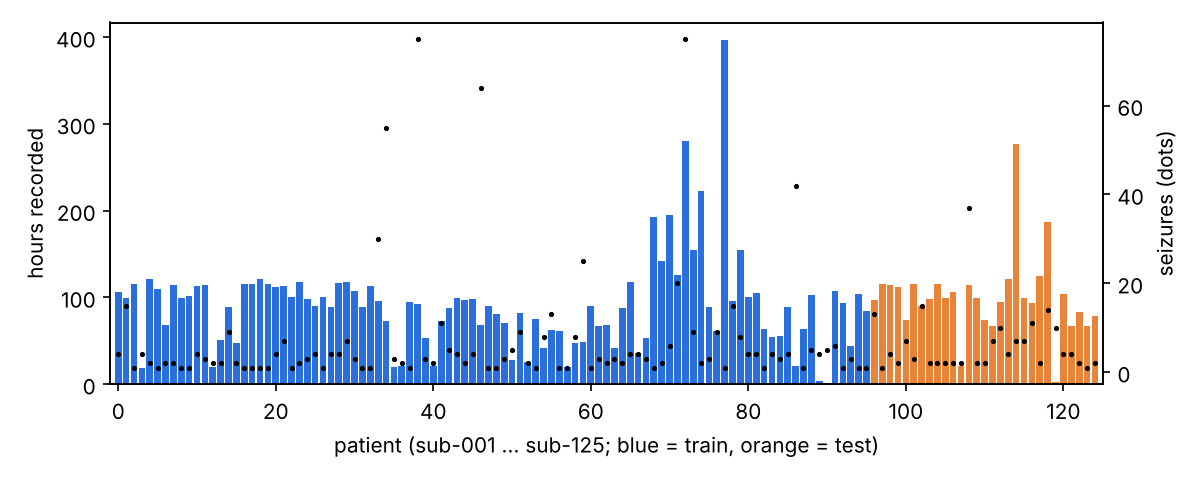
\includegraphics[width=0.9\textwidth]{figures/hours_and_seizures_per_patient.png}
\caption{Hours recorded (bars; blue: training, orange: test) and seizures per patient (dots).}\label{fig:hours}
\end{figure}

\section{Audit Findings}

\begin{table}[H]
\centering\small
\caption{Where the released files differ from the documentation, and what we did.}\label{tab:docdiff}
\begin{tabularx}{\textwidth}{@{}P{38mm}P{26mm}P{30mm}L@{}}
\toprule
\textbf{Item} & \textbf{Documentation} & \textbf{Files} & \textbf{Action}\\
\midrule
Sampling rate & 250 Hz & 256 Hz & Filters designed for 256 Hz\\
Seizures & 886 & 883 & Report our count\\
Centre and age labels & used for splits & not released & Folds by seizure count\\
Official artefact rule & 13--150\,\textmu V & flags 69\,\% of normal windows & Flags used as input bits\\
Downloads & -- & 9 files cut short & Size checks; re-extracted\\
Evaluation code & -- & two defects & Corrected values reported alongside\\
\bottomrule
\end{tabularx}
\end{table}

\section{System Architecture}

\begin{figure}[H]
\centering
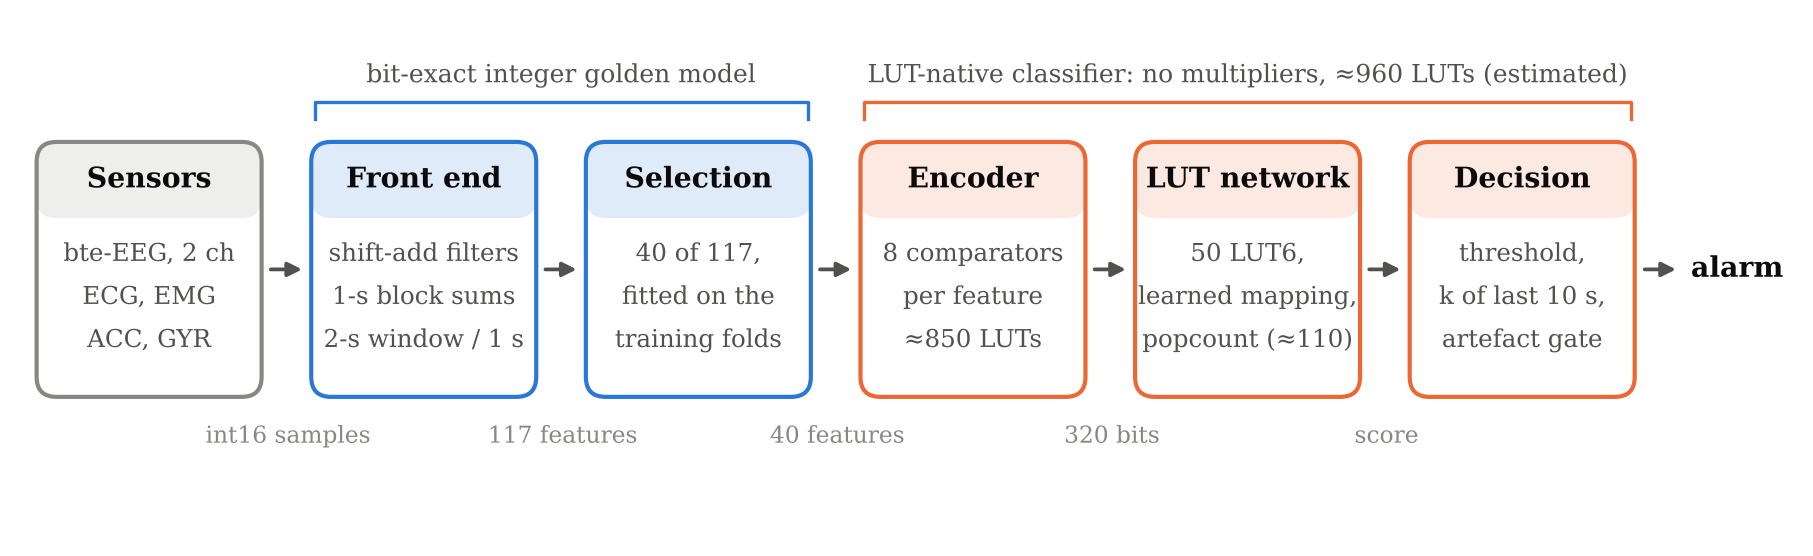
\includegraphics[width=\textwidth]{figures/system_overview.png}
\caption{The proposed detector. Blue: bit-exact integer front end; orange: LUT-native classifier.}\label{fig:system}
\end{figure}

\begin{itemize}
\item Every second, the last 2 s of all signals become \textbf{117 integer features} (Table~\ref{tab:features}).
\item The 40 most useful features are thermometer-encoded and classified by a \textbf{50-neuron LUT network}.
\item An alarm is raised when at least $k$ of the last 10 seconds are positive.
\end{itemize}

\begin{table}[H]
\centering\small
\caption{The 117 integer features (per 2-s window; many also as change from a 64-s moving average).}\label{tab:features}
\begin{tabularx}{\textwidth}{@{}lcL@{}}
\toprule
\textbf{Group} & \textbf{Count} & \textbf{Features}\\
\midrule
EEG & 84 & amplitude, line length, mobility, zero crossings, extrema, 5 band amplitudes; artefact flags\\
ECG & 5 & log heart period, log RR variability, quality flag\\
EMG & 8 & amplitude, line length, zero crossings, high/low band ratio\\
Motion & 16 & accelerometer and gyroscope magnitude, jerk, activity, band amplitude\\
Presence & 4 & one bit per sensor (ECG, EMG, accelerometer, gyroscope)\\
\bottomrule
\end{tabularx}
\end{table}

\paragraph{Integer arithmetic.} Filters use coefficients that are sums of powers of two (shifts and adds only), with
error feedback; heart rate uses $\log_2(\mathrm{RR})$, so there is no division. On the board the same front end runs in the
FPGA fabric as a microcoded shift-add engine (Section~\ref{sec:fe-engine}). A floating-point twin measures the cost
of the integer arithmetic (Section~\ref{sec:intfloat}).

\section{The LUT-Native Classifier (DWN)}

A Differentiable Weightless Neural Network \cite{bacellar2024dwn} has no weights: each neuron is a 6-input truth table,
exactly one FPGA LUT.
\begin{equation}
  b_{f,i} = [\,x_f > t_{f,i}\,],\quad i = 1,\dots,8 \qquad\qquad s = \sum_{j \in S} y_j - \sum_{j \in B} y_j
\end{equation}
Each feature becomes 8 thermometer bits (one comparator each); each neuron reads 6 learned bits and outputs one stored
bit $y_j$; the score $s$ is the popcount of the seizure group $S$ minus that of the background group $B$.
Figure~\ref{fig:cost} shows the hardware cost of the final network.

\begin{figure}[H]
\centering
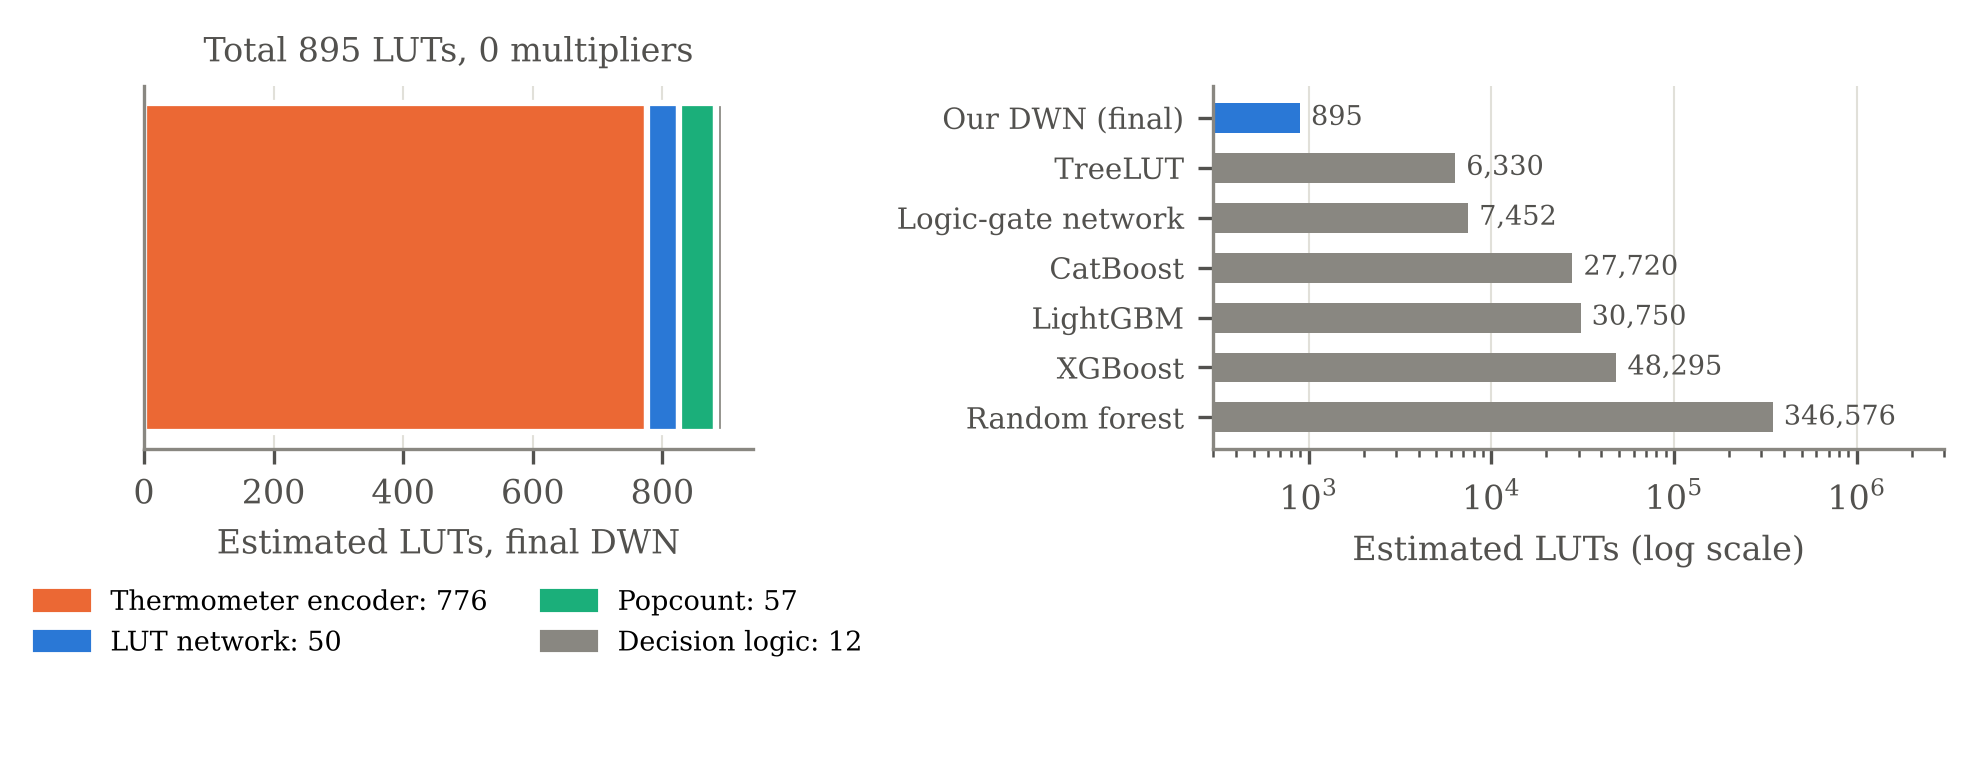
\includegraphics[width=\textwidth]{figures/cost.png}
\caption{Estimated hardware cost. Left: the final DWN by block (the encoder dominates). Right: total LUTs of each model,
log scale.}\label{fig:cost}
\end{figure}

\section{Models and Extensions}

\begin{table}[H]
\centering\small
\caption{Models compared on the same features, splits and metrics.}\label{tab:models}
\begin{tabularx}{\textwidth}{@{}P{36mm}L@{}}
\toprule
\textbf{Group} & \textbf{Models}\\
\midrule
Published baselines & ChronoNet \cite{roy2019chrononet} (CNN + GRU on raw EEG); SVM \cite{vandecasteele2020bte}\\
Software references & logistic regression, random forest, XGBoost, LightGBM, CatBoost\\
Hardware-oriented & INT8 MLP (multipliers), TreeLUT \cite{khataei2025treelut}, logic-gate network \cite{petersen2022dlgn}, DWN \cite{bacellar2024dwn}\\
\bottomrule
\end{tabularx}
\end{table}

\begin{table}[H]
\centering\small
\caption{Extensions of the DWN tested in this project (adopted only if significantly better).}\label{tab:extensions}
\begin{tabularx}{\textwidth}{@{}cL@{}}
\toprule
\textbf{ID} & \textbf{Idea}\\
\midrule
N1 & Memory across seconds: 16 state bits fed back; stacked past windows\\
N2 & Encoder design: uniform, Gaussian and learned thresholds\\
N3 & Label-free per-patient threshold adaptation\\
N4 & Distillation from LightGBM; teacher-guided hard negatives\\
N5 & Focal, noise-robust (GCE, SCE) and multiple-instance losses; onset weighting\\
N6 & Modality dropout, gated fusion, late fusion\\
N7 & Interpretability: which inputs the LUTs read during alarms\\
N8 & Post-ictal verification: a second LUT network confirms each alarm (secondary analysis)\\
\bottomrule
\end{tabularx}
\end{table}

\section{Evaluation Protocol}\label{sec:eval}

\begin{itemize}
\item \textbf{Patient-wise 5-fold cross-validation} on the 96 training patients for every design choice.
\item \textbf{Sealed test set}: the 29 test patients scored once, after the freeze, with 5 seeds; every access logged.
\item \textbf{SzCORE event scoring} \cite{dan2024szcore} (30\,s before, 60\,s after, 90\,s merge), per patient:
\end{itemize}
\begin{equation}
  \mathrm{Sens} = \frac{TP}{TP + FN},\qquad \mathrm{Prec} = \frac{TP}{TP + FP},\qquad
  F_1 = \frac{2\,\mathrm{Sens}\cdot\mathrm{Prec}}{\mathrm{Sens} + \mathrm{Prec}},\qquad \text{false alarms per 24 h}
\end{equation}
\begin{itemize}
\item \textbf{Operating points} (threshold, $k$, artefact gate) chosen on the training folds: best event-F1, and highest
  sensitivity with at most one false alarm per hour.
\item \textbf{Statistics}: paired Wilcoxon test per patient; an extension is adopted only if $p < 0.05$ in its favour.
\item \textbf{Paper metrics} (the base paper's own code) are reported for the comparison with the base paper.
\item \textbf{Compute}: a 4-core CPU server and a laptop RTX 3060 GPU.
\end{itemize}

\chapter{Experimental Results and Comparisons}\label{ch:results}

Sections~\ref{sec:res-chrononet}--\ref{sec:res-types}: development on the 96 training patients
(patient-wise cross-validation). Sections~\ref{sec:res-test}--\ref{sec:res-hw}: the single evaluation on the 29
held-out test patients, after the design was frozen.

\section{Reproduction of the Published Baseline}\label{sec:res-chrononet}

\begin{figure}[H]
\centering
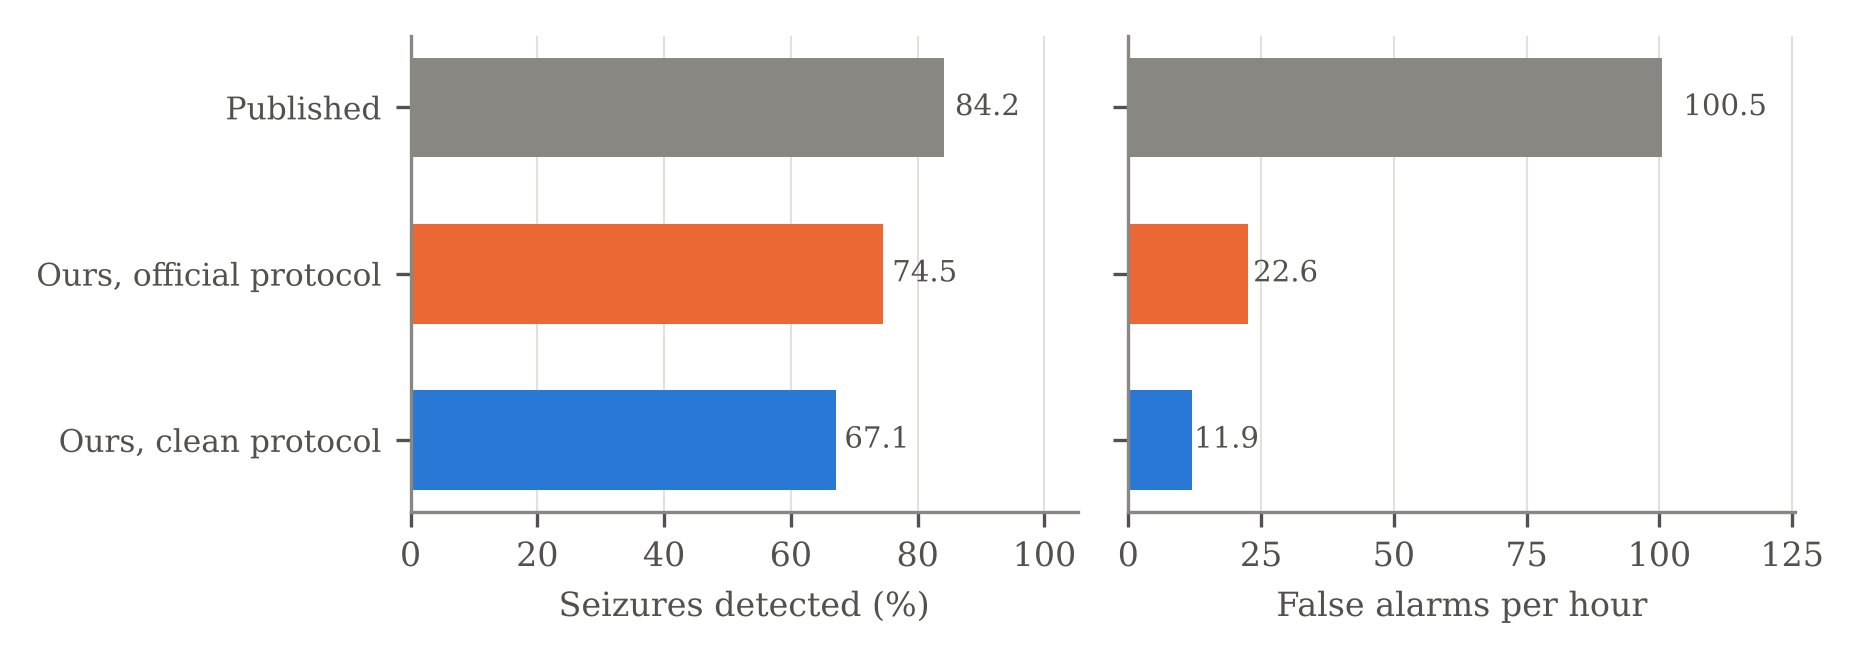
\includegraphics[width=0.9\textwidth]{figures/chrononet_repro.png}
\caption{ChronoNet on the 29 test patients: published and reproduced (the paper's metrics).}\label{fig:chrononet}
\end{figure}

\begin{itemize}
\item \textbf{Partly reproduced}: 74.5\,\% of seizures detected against 84.2\,\% published, with 22.6 instead of 100.5
  false alarms per hour (Figure~\ref{fig:chrononet}); the per-recording AUPR matches (0.109 vs 0.104).
\item \textbf{Test-set leak}: the released code picks its training epoch on the test patients. Our \textbf{clean} run
  (last epoch, no test information: 67.1\,\%, 11.9 false alarms/h) is the reference for the final comparison.
\end{itemize}

\section{Integer Versus Floating-Point Features}\label{sec:intfloat}

\begin{table}[H]
\centering\small
\caption{The integer front end against its floating-point twin (10 training patients).}\label{tab:intfloat}
\begin{tabular}{@{}lc@{}}
\toprule
\textbf{Check} & \textbf{Result}\\
\midrule
Median feature correlation, integer vs float & 0.9965\\
Artefact flags agreeing & 99.7\,\%\\
LightGBM AUROC, integer vs float features & 0.736 vs 0.735\\
\bottomrule
\end{tabular}
\end{table}

\section{Comparison of Model Families}\label{sec:res-families}

\begin{table}[H]
\centering\small
\caption{Five-fold cross-validation on the 96 training patients (best-F1 operating point).}\label{tab:families}
\begin{tabularx}{\textwidth}{@{}P{38mm}ccccL@{}}
\toprule
\textbf{Model} & \textbf{AUROC} & \textbf{Event-F1} & \textbf{FA / 24 h} & \textbf{Sens.\ at $\le$1 FA/h} & \textbf{Estimated cost}\\
\midrule
LightGBM & 0.870 & 0.292 & 3.6 & 0.594 & $\approx$30.6k LUTs\\
CatBoost & 0.863 & 0.286 & 3.0 & 0.618 & $\approx$27.7k LUTs\\
XGBoost & 0.867 & 0.277 & 3.4 & 0.603 & $\approx$47.9k LUTs\\
TreeLUT & 0.857 & 0.266 & 4.2 & 0.619 & $\approx$6.4k LUTs\\
\textbf{DWN + distillation (final)} & 0.851 & \textbf{0.229} & \textbf{0.9} & 0.597 & \textbf{$\approx$870 LUTs}\\
DWN base & 0.840 & 0.211 & 2.4 & 0.581 & $\approx$960 LUTs\\
Random forest & 0.852 & 0.198 & 0.5 & 0.536 & $\approx$323k LUTs\\
Logic-gate network & 0.843 & 0.171 & 4.9 & 0.540 & $\approx$7.5k LUTs\\
INT8 MLP & 0.830 & 0.147 & 7.8 & 0.520 & 9,600 multiplications\\
Logistic regression & 0.806 & 0.105 & 8.8 & 0.409 & 117 multiplications\\
\bottomrule
\end{tabularx}
\end{table}

\begin{figure}[H]
\centering
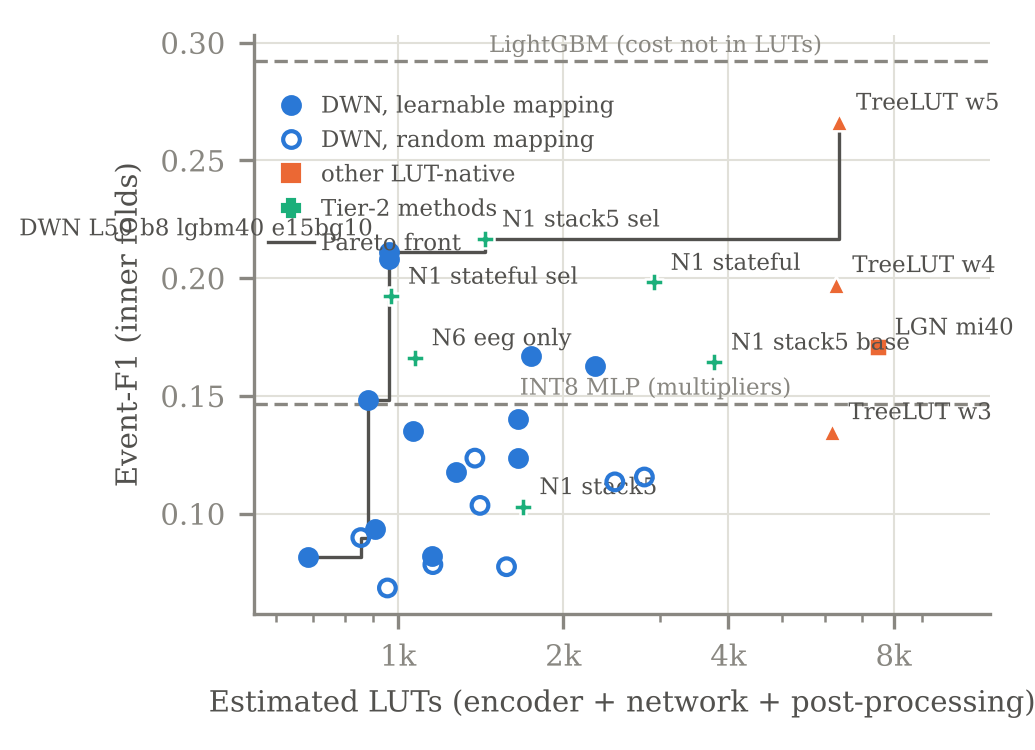
\includegraphics[width=0.68\textwidth]{figures/pareto_inner_cv.png}
\caption{Event-F1 against estimated LUTs for every LUT-native run (training folds), with the Pareto front.}\label{fig:pareto}
\end{figure}

\paragraph{Findings.} The DWN is 7--8$\times$ smaller than the other LUT models and beats the INT8 MLP on every metric
(Table~\ref{tab:families}). Larger networks (up to 2,000 LUTs), 16 thresholds, two layers and other temperatures gave no
significant gain (Figure~\ref{fig:pareto}); 4-input LUTs and 4 thresholds were clearly worse.

\section{What Improved the Network}\label{sec:res-ext}

\begin{figure}[H]
\centering
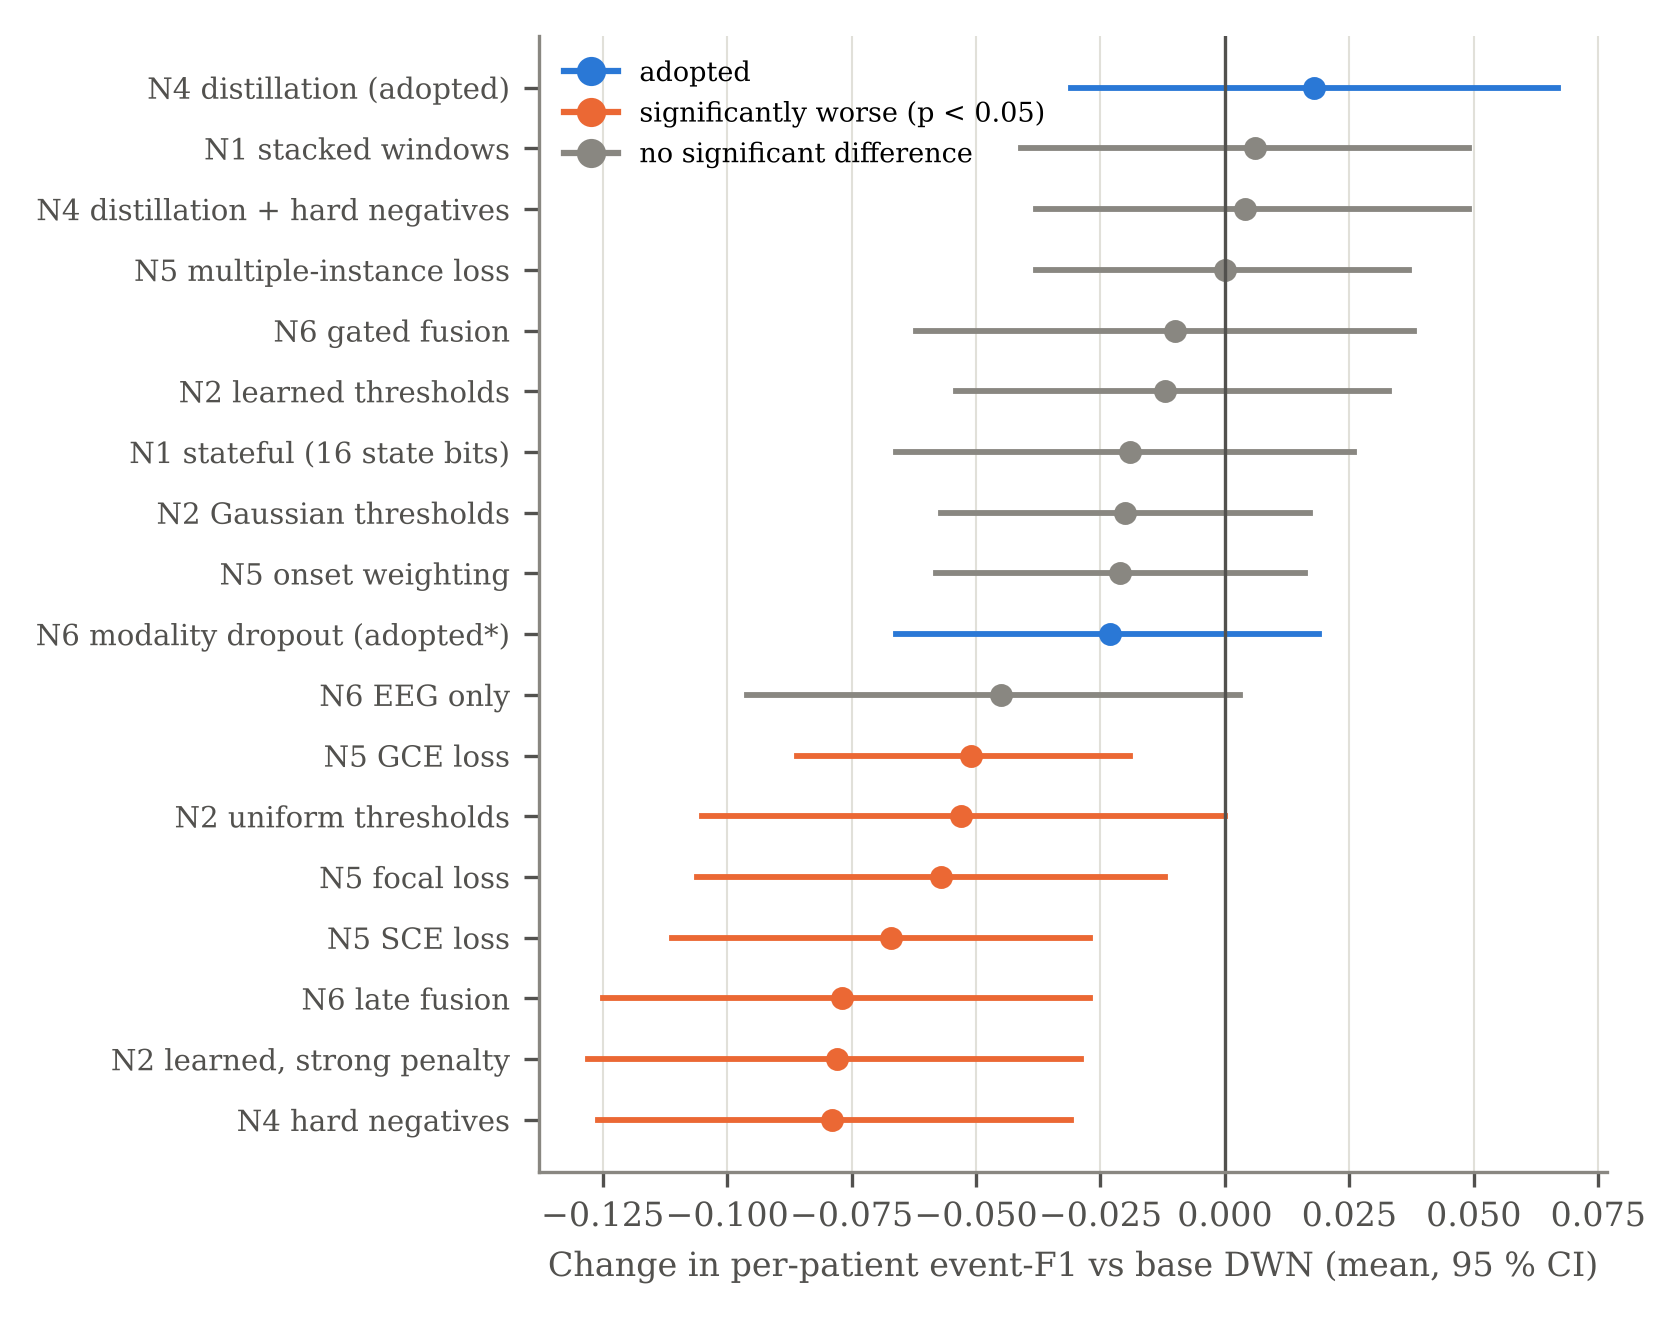
\includegraphics[width=0.85\textwidth]{figures/ablation.png}
\caption{Every extension against the base DWN: mean change in per-patient event-F1 with 95\,\% interval. *Modality
dropout was adopted for its robustness to missing sensors (Section~\ref{sec:res-missing}).}\label{fig:ablation}
\end{figure}

\begin{table}[H]
\centering\small
\caption{The changes that passed the significance test.}\label{tab:adopted}
\begin{tabularx}{\textwidth}{@{}P{42mm}LP{38mm}@{}}
\toprule
\textbf{Change} & \textbf{Evidence (training patients)} & \textbf{How it was found}\\
\midrule
Feature selection by LightGBM importance & event-F1 0.148 $\to$ 0.208 ($p = 0.047$); false alarms 7.0 $\to$ 2.3/day & N7 showed the network ignored heart rate\\
Distillation from LightGBM (\textbf{final}) & false alarms 2.4 $\to$ 0.9/day ($p = 3\times10^{-7}$); event-F1 0.229 vs 0.211 & N4\\
Modality dropout (variant) & without ECG: event-F1 0.092 $\to$ 0.172 ($p = 0.005$) & N6\\
\bottomrule
\end{tabularx}
\end{table}

\begin{figure}[H]
\centering
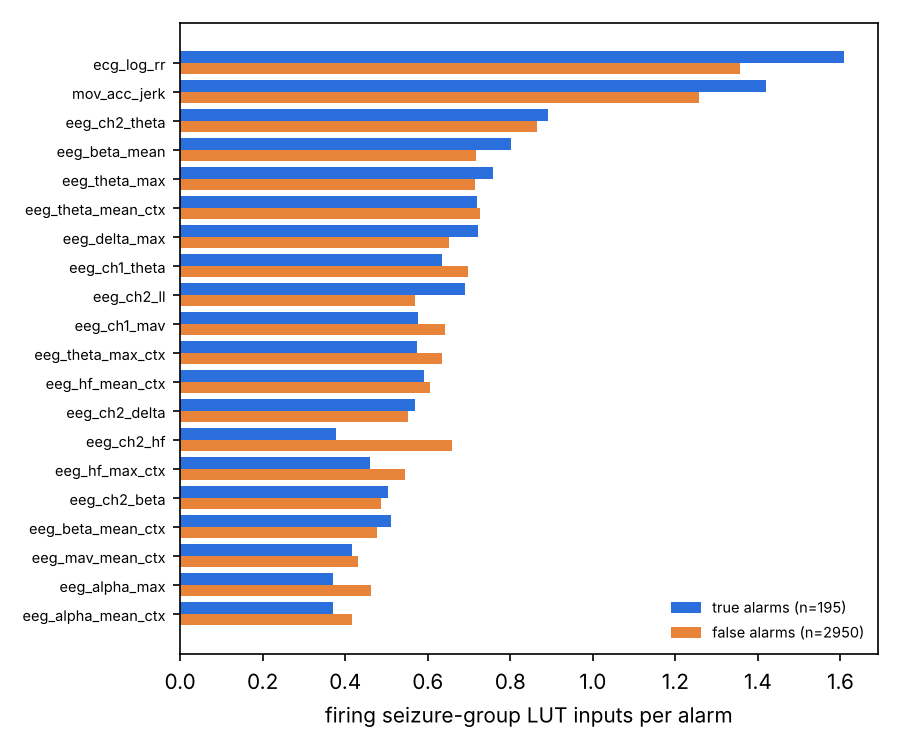
\includegraphics[width=0.55\textwidth]{figures/n7_feature_usage.png}
\caption{N7: inputs read by the firing seizure LUTs during true and false alarms (first, mutual-information network):
false alarms look like seizures to it.}\label{fig:n7}
\end{figure}

\section{Missing Sensors}\label{sec:res-missing}

\begin{figure}[H]
\centering
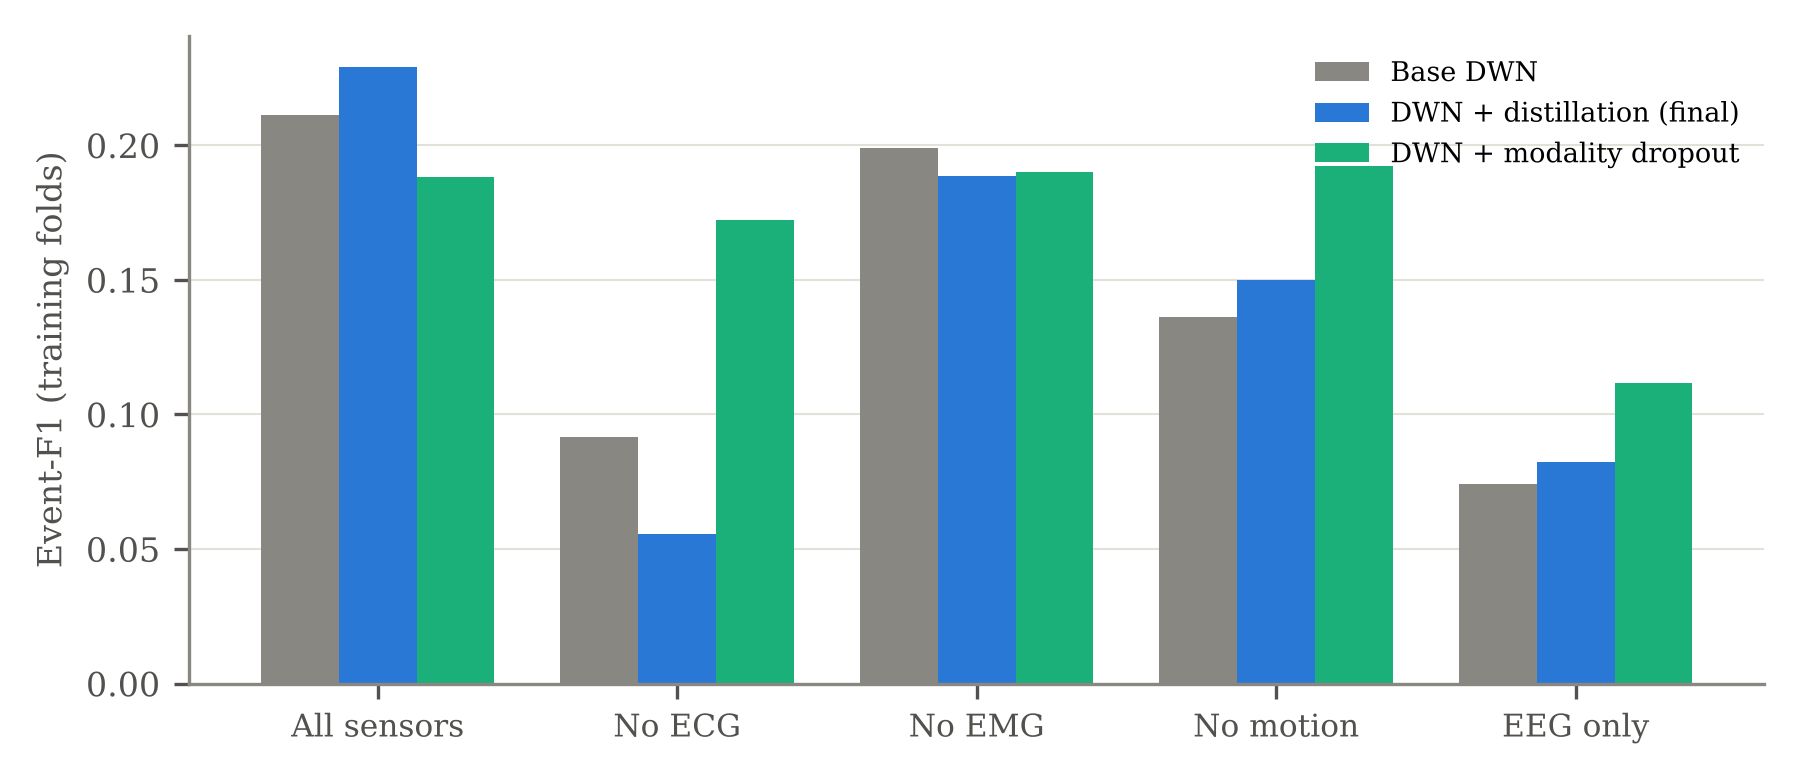
\includegraphics[width=0.85\textwidth]{figures/missing_sensors.png}
\caption{Event-F1 with sensors removed at test time (training folds). Distillation is the most accurate with all
sensors; modality dropout keeps working without ECG or motion.}\label{fig:missing}
\end{figure}

\section{Seizure Types}\label{sec:res-types}

\begin{figure}[H]
\centering
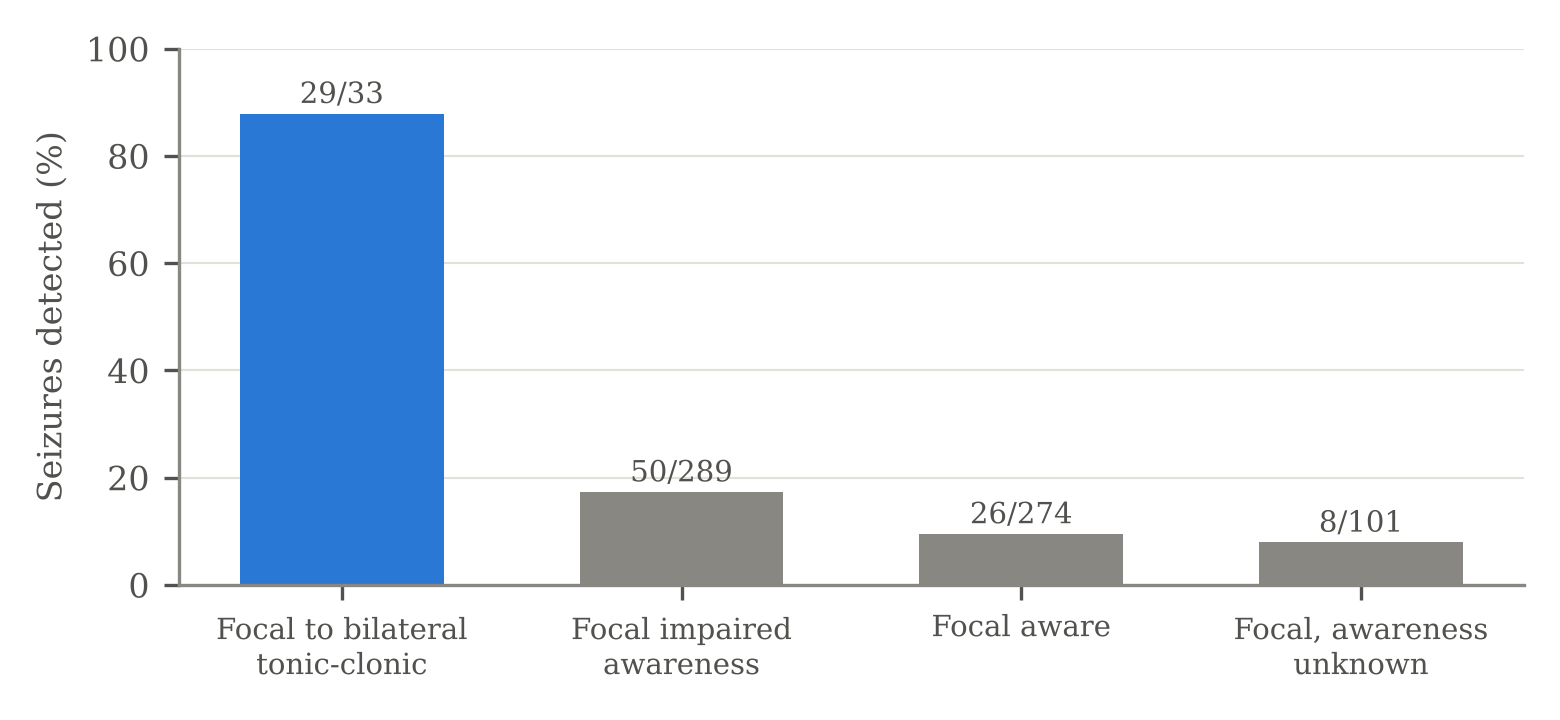
\includegraphics[width=0.65\textwidth]{figures/seizure_types.png}
\caption{Seizures detected by type (base DWN, training folds): tonic-clonic seizures are caught, focal seizures rarely.}\label{fig:types}
\end{figure}

\section{Final Evaluation on the Held-Out Test Patients}\label{sec:res-test}

\begin{figure}[H]
\centering
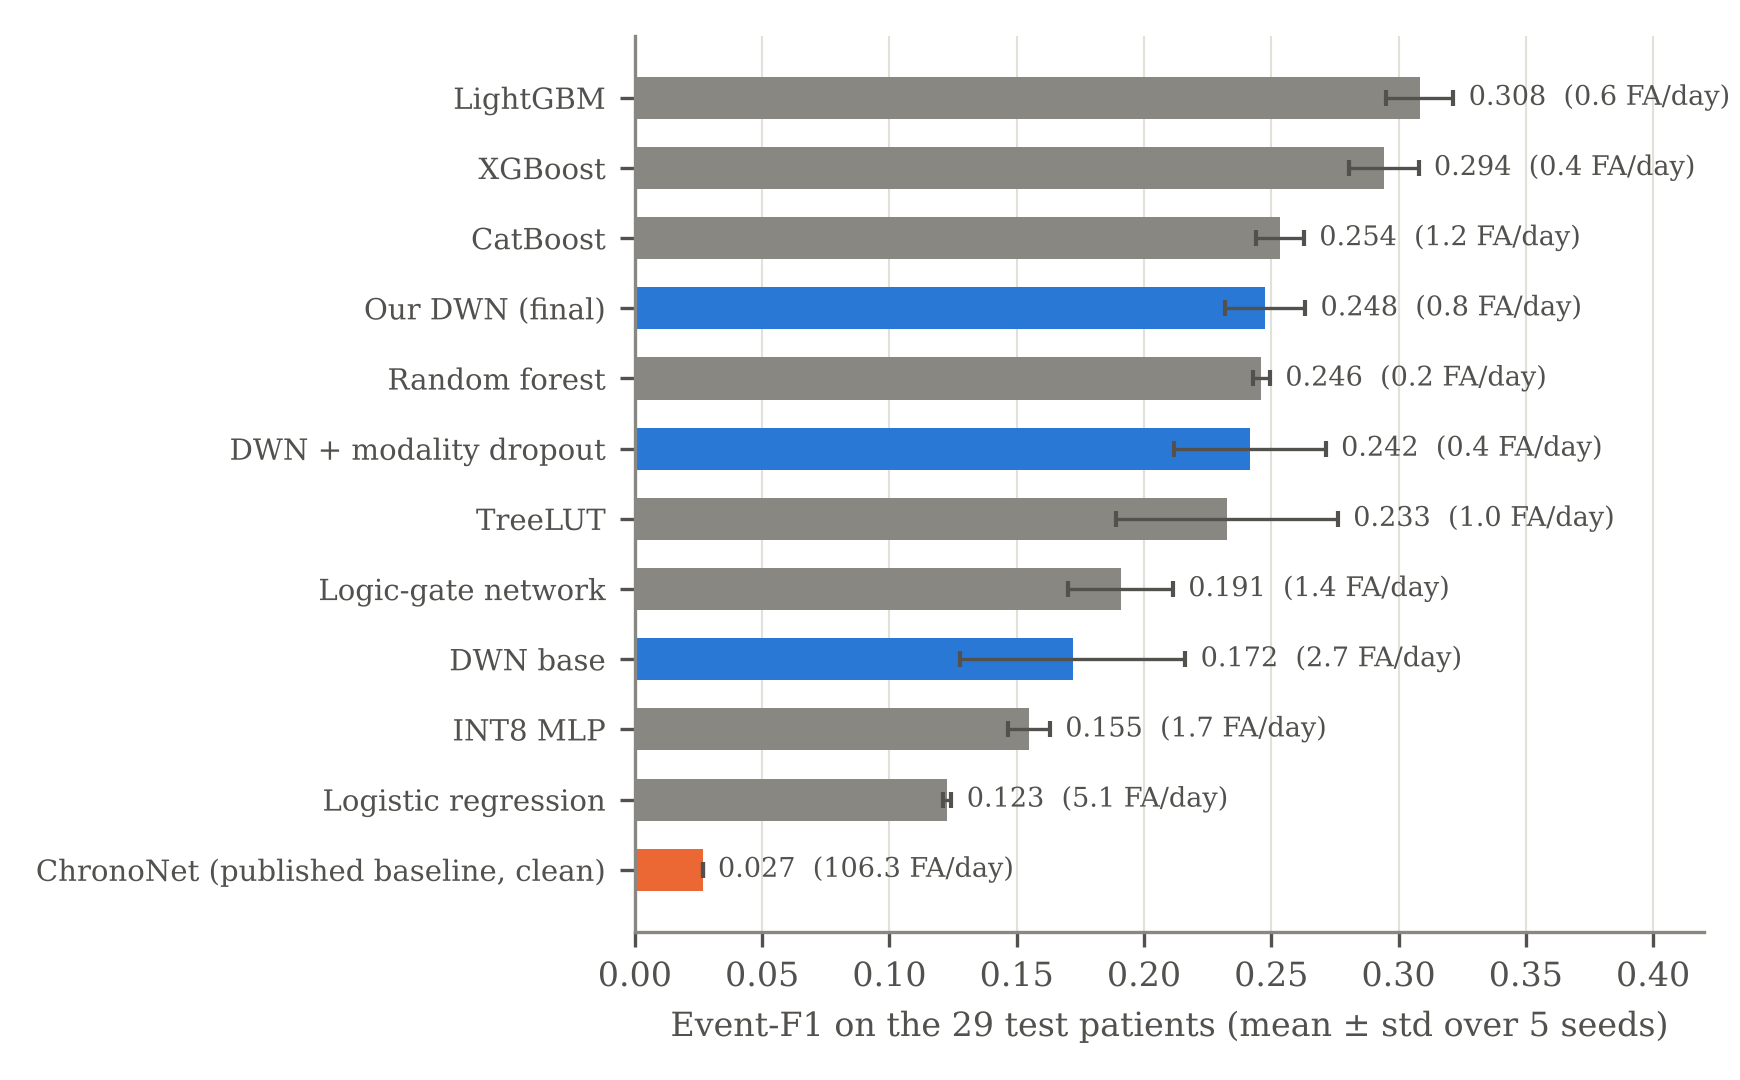
\includegraphics[width=0.85\textwidth]{figures/test_f1.png}
\caption{Event-F1 on the 29 test patients (mean $\pm$ std over 5 seeds) and false alarms per day.}\label{fig:testf1}
\end{figure}

\begin{figure}[H]
\centering
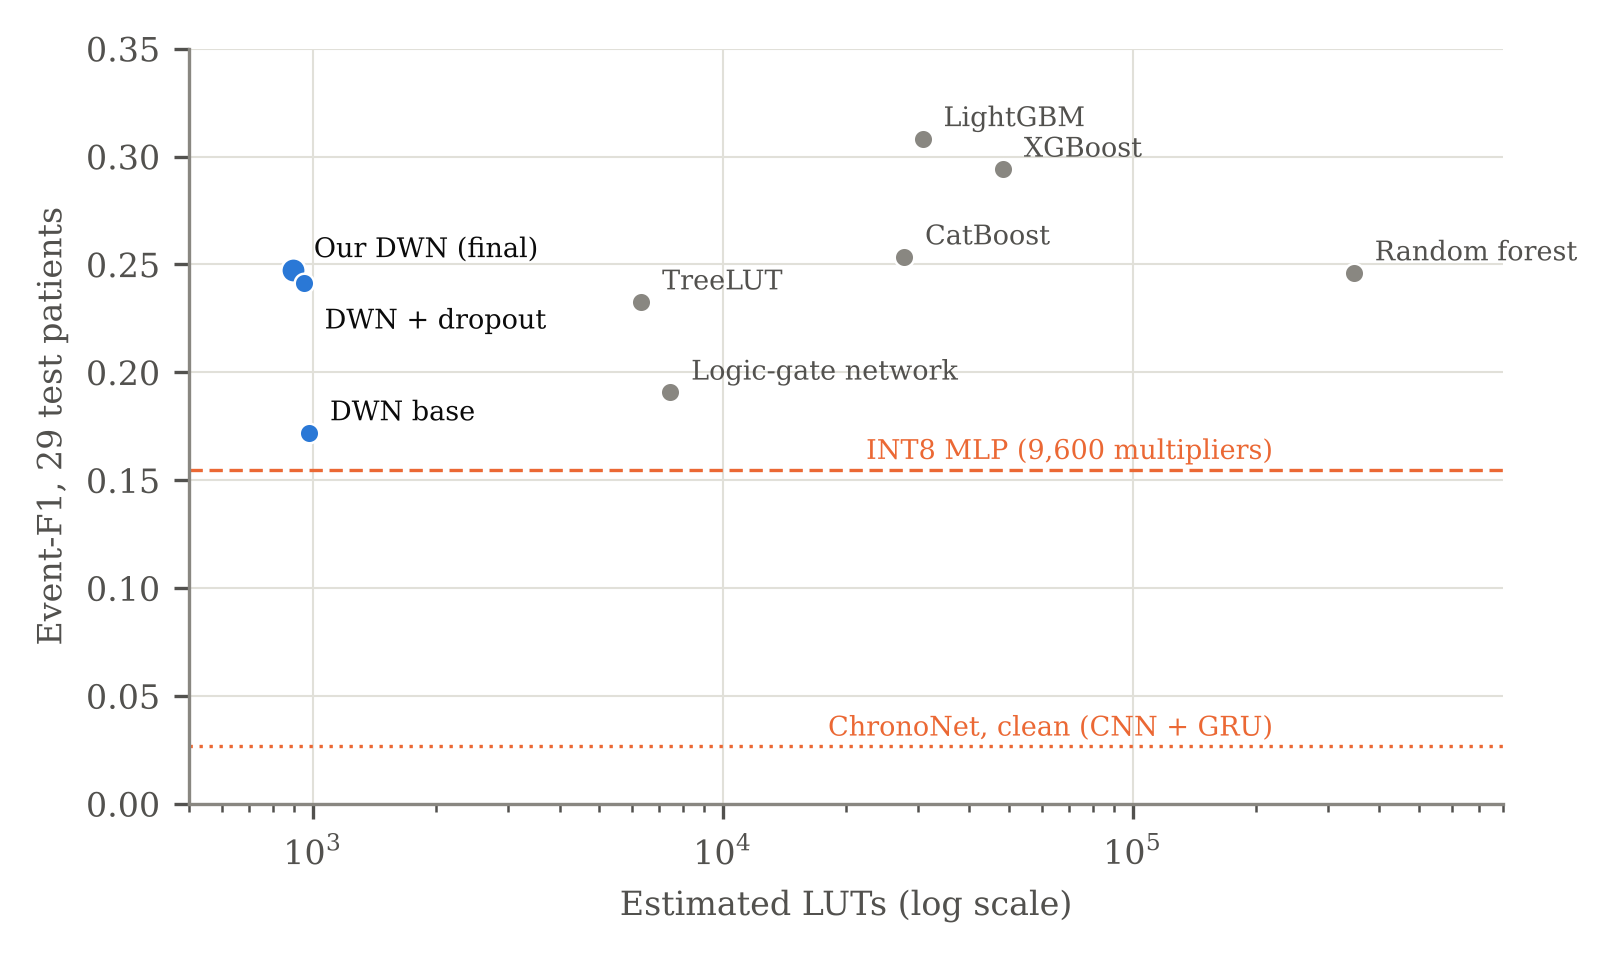
\includegraphics[width=0.8\textwidth]{figures/test_f1_vs_luts.png}
\caption{Accuracy against hardware cost on the test patients: the LUT networks reach tree-ensemble accuracy at a
fraction of the LUTs.}\label{fig:testluts}
\end{figure}

\begin{table}[H]
\centering\small
\caption[Final DWN against the main references on the 29 test patients.]{Final DWN against the main references on the 29 test patients ($p$: paired Wilcoxon on per-patient event-F1).}\label{tab:test}
\begin{tabularx}{\textwidth}{@{}P{40mm}cccL@{}}
\toprule
\textbf{Model} & \textbf{Event-F1} & \textbf{FA / 24 h} & \textbf{$p$ vs ChronoNet} & \textbf{Estimated cost}\\
\midrule
\textbf{DWN + distillation (final)} & \textbf{0.248 $\pm$ 0.016} & \textbf{0.8} & 0.027 & \textbf{$\approx$900 LUTs}\\
LightGBM & 0.308 $\pm$ 0.013 & 0.6 & 0.027 & $\approx$30.8k LUTs\\
CatBoost & 0.254 $\pm$ 0.009 & 1.2 & 0.031 & $\approx$27.7k LUTs\\
Random forest & 0.246 $\pm$ 0.003 & 0.2 & 0.27 & $\approx$347k LUTs\\
TreeLUT & 0.233 $\pm$ 0.044 & 1.0 & 0.016 & $\approx$6.3k LUTs\\
Logic-gate network & 0.191 $\pm$ 0.021 & 1.4 & 0.034 & $\approx$7.5k LUTs\\
INT8 MLP & 0.155 $\pm$ 0.008 & 1.7 & 0.017 & 9,600 multiplications\\
ChronoNet (clean) & 0.027 & 106 & -- & CNN + GRU\\
\bottomrule
\end{tabularx}
\end{table}

\paragraph{Findings.} The result held on unseen patients (0.248, above the cross-validation 0.229). The final DWN scores
above TreeLUT, the logic-gate network and the INT8 MLP, is level with random forest and CatBoost at 30--390$\times$ fewer
LUTs, and is significantly better than ChronoNet; LightGBM remains ahead ($p = 0.039$). All 11 models are in
Table~\ref{tab:test-full} (Appendix~\ref{app:sources}).

\section{Comparison with the Base Paper}\label{sec:res-published}

\begin{figure}[H]
\centering
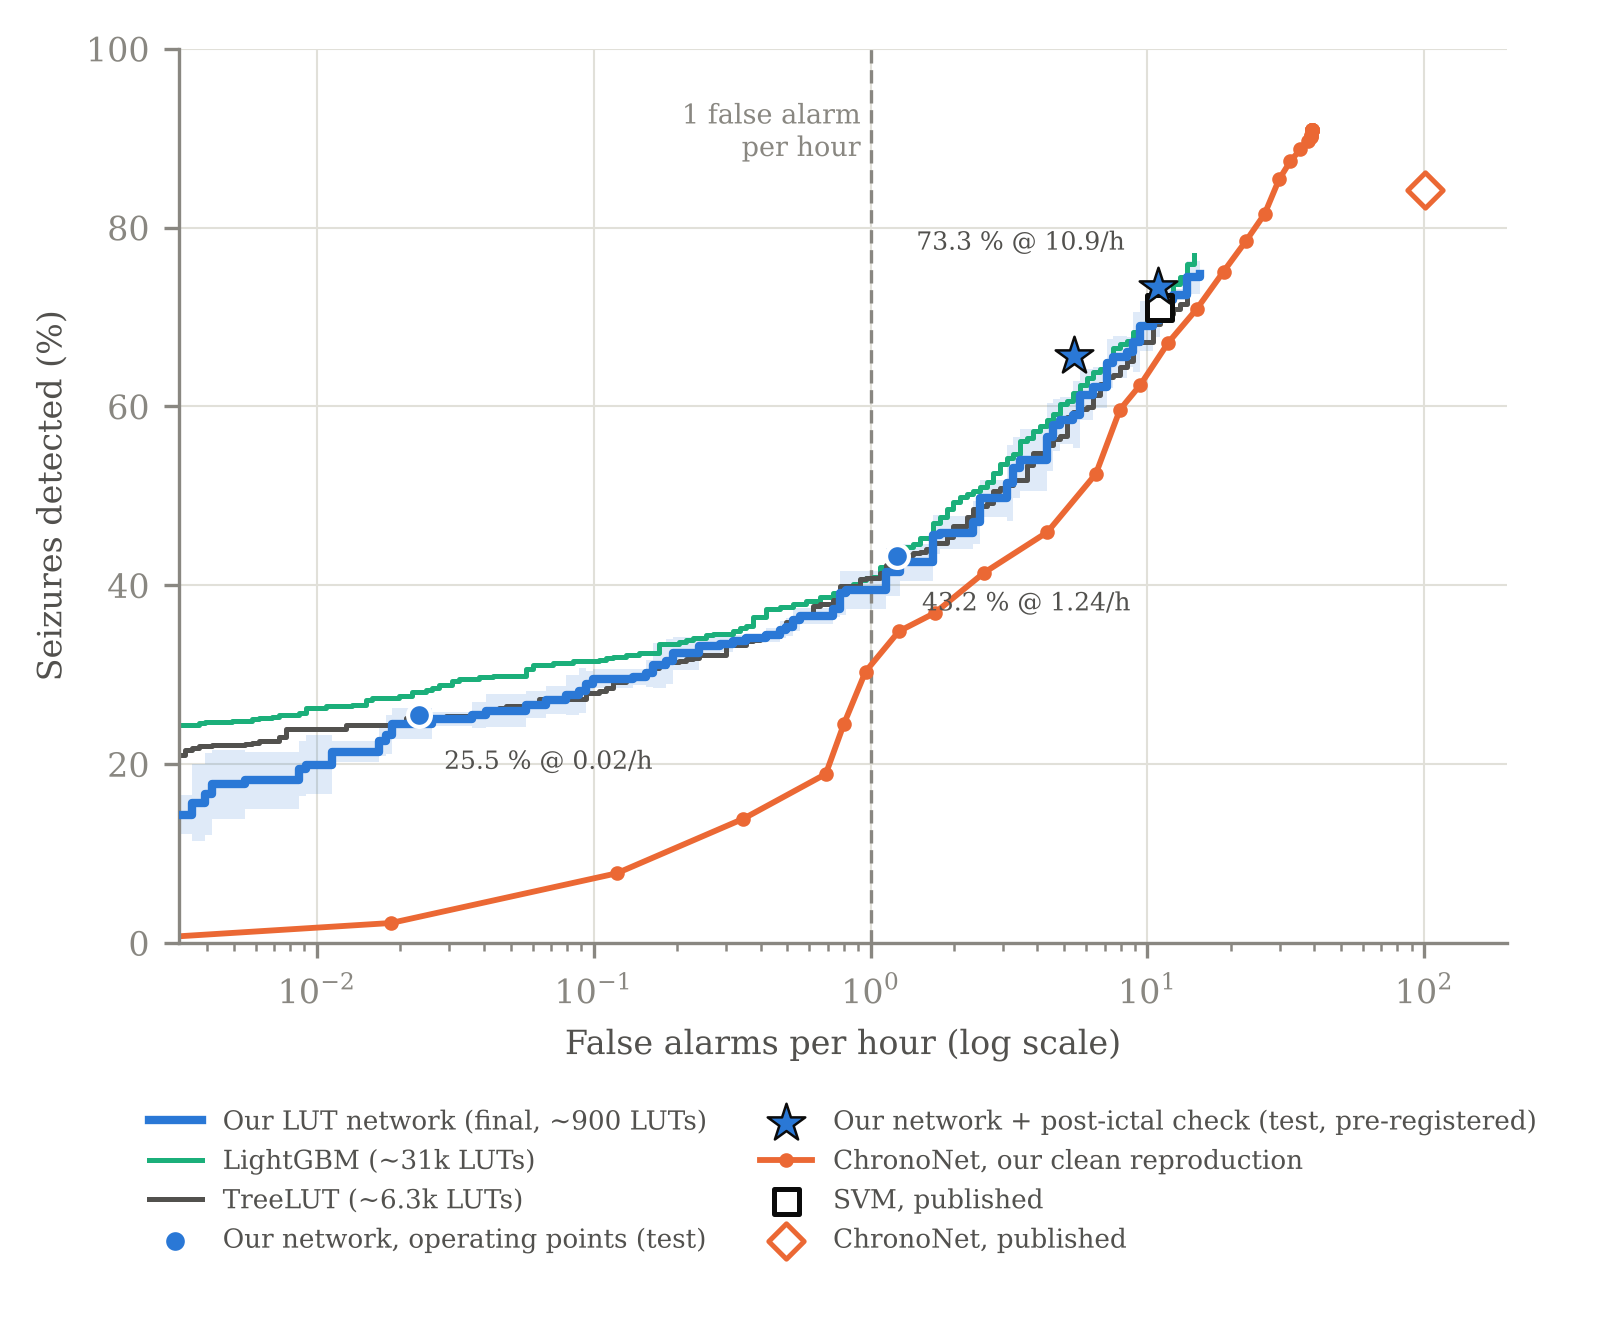
\includegraphics[width=0.85\textwidth]{figures/sens_fa_test.png}
\caption{Seizures detected against false alarms per hour on the 29 test patients (the base paper's metrics). Curves:
threshold sweeps of the frozen models (mean of 5 seeds; band: std of our network), drawn as far as every seed's sweep
reaches; dots: our two operating points, chosen on the training folds; stars: the two-stage detector
(Section~\ref{sec:res-n8}); open markers: published values.}\label{fig:sensfa}
\end{figure}

\begin{table}[H]
\centering\small
\caption{The base paper's baselines and our network on the same 29 test patients (the paper's metrics).}\label{tab:published}
\begin{tabularx}{\textwidth}{@{}P{70mm}ccL@{}}
\toprule
\textbf{Model} & \textbf{Detected} & \textbf{FA / h} & \textbf{AUROC}\\
\midrule
SVM, published \cite{bhagubai2025seizeit2} & 71.1\,\% & 11.0 & 0.700\\
ChronoNet, published \cite{bhagubai2025seizeit2} & 84.2\,\% & 100.5 & 0.792\\
ChronoNet, our clean reproduction & 67.1\,\% & 11.9 & 0.746\\
ChronoNet at $\approx$1.3 FA/h$^{*}$ & 34.8\,\% & 1.26 & --\\
\textbf{Our DWN, $\le$1 FA/h operating point} & \textbf{43.2\,\%} & \textbf{1.24} & \textbf{0.883}\\
\textbf{Our DWN, best-F1 operating point} & \textbf{25.5\,\%} & \textbf{0.02} & \\
\textbf{Our DWN + post-ictal check (pre-registered)$^{\dagger}$} & \textbf{73.3\,\%} & \textbf{10.9} & \\
\textbf{Same, stricter verification$^{\dagger}$} & \textbf{65.6\,\%} & \textbf{5.4} & \\
\bottomrule
\multicolumn{4}{@{}p{\textwidth}@{}}{\footnotesize $^{*}$ threshold read from ChronoNet's own test curve (favours it); at
0.02 FA/h ChronoNet detects 2.2\,\%. AUROC pooled over test windows; the published 0.792 uses an unreproduced definition.
$^{\dagger}$ Secondary analysis after the final test (Section~\ref{sec:res-n8}); 96\,s decision delay.}
\end{tabularx}
\end{table}

\paragraph{Findings.} The paper's baselines run at 11--100 false alarms per hour. At the same false-alarm rate our
network detects more seizures than ChronoNet (43.2\,\% vs 34.8\,\% at $\approx$1.25/h; 25.5\,\% vs 2.2\,\% at
$\approx$0.02/h), ranks windows better (AUROC 0.883 vs 0.746), and needs no multipliers. At the SVM's rate of 11 false
alarms per hour its curve reaches 69.7\,\% (SVM, published: 71.1\,\%), level with LightGBM (70.5\,\%) at 3\,\% of its
LUTs; this value is read from the test curve itself and is therefore optimistic.

\section{Post-Ictal Verification (Secondary Analysis)}\label{sec:res-n8}

Requested after the final test: detect more seizures than the base paper at slightly fewer false alarms. A two-stage
detector (N8) runs the final network at a sensitive threshold and confirms each alarm 96\,s later with a second LUT
network (50 LUTs) that compares the alarm with the minutes before and after it (EEG, heart rate, EMG, motion). All
settings were chosen on the training patients and committed before one evaluation on the test patients.

\begin{table}[H]
\centering\small
\caption[Two-stage detector with post-ictal verification.]{Two-stage detector: training patients (cross-validation) and test patients (5 seeds, paper's metrics).}\label{tab:n8}
\begin{tabular}{@{}lcccc@{}}
\toprule
\textbf{Detector} & \multicolumn{2}{c}{\textbf{Training (CV)}} & \multicolumn{2}{c}{\textbf{Test}}\\
 & Detected & FA/h & Detected & FA/h\\
\midrule
Final network, lower threshold & 74.2\,\% & 8.5 & 66.4 $\pm$ 2.0\,\% & 7.6\\
\textbf{+ post-ictal check ($\le$10 FA/h)} & 81.9\,\% & 9.6 & \textbf{73.3 $\pm$ 1.4\,\%} & \textbf{10.9}\\
+ post-ictal check ($\le$5 FA/h) & 72.3\,\% & 4.8 & 65.6 $\pm$ 1.0\,\% & 5.4\\
SVM, published \cite{bhagubai2025seizeit2} & -- & -- & 71.1\,\% & 11.0\\
\bottomrule
\end{tabular}
\end{table}

\paragraph{Findings.} At the SVM's false-alarm rate (10.9 vs 11.0 per hour) the LUT-native two-stage detector detects
2.2 points more seizures (all 5 seeds above 71.1\,\%; a small margin against a single published value). Verification
adds 3.6--6.5 points over the network alone at the same false-alarm rate. Costs: a 96\,s decision delay (seizure
logging, not instant alarms) and many false alarms per day, as for the paper's baselines; the low-false-alarm result of
Section~\ref{sec:res-test} remains the primary one.

\section{Hardware Handoff Check}\label{sec:res-hw}

\begin{table}[H]
\centering\small
\caption{Verilog of the final DWN against the software on 10 test recordings.}\label{tab:verilog}
\begin{tabular}{@{}ll@{}}
\toprule
\textbf{Item} & \textbf{Result}\\
\midrule
Exported & thresholds, input mapping, 50 truth tables, popcount head\\
Test vectors & raw samples, features, bits, LUT outputs, scores, alarms\\
Windows simulated (Icarus Verilog) & 431,960\\
Mismatches & \textbf{0}\\
\bottomrule
\end{tabular}
\end{table}

\chapter{FPGA Implementation, Self-Test and Board Results}\label{ch:hw}

\section{System on the Kria KV260}

The detector runs on an AMD Kria KV260 board (Zynq UltraScale+ XCK26: four Arm Cortex-A53 cores and FPGA fabric).
In the final design (kit v6) the Arm cores only move raw samples; the front end and the classifier both run in the
fabric (Figure~\ref{fig:arch}).

\begin{figure}[H]
\centering
\resizebox{\textwidth}{!}{% SeizeLUT on the KV260 (kit v6): processing system (Arm) and programmable logic (fabric)
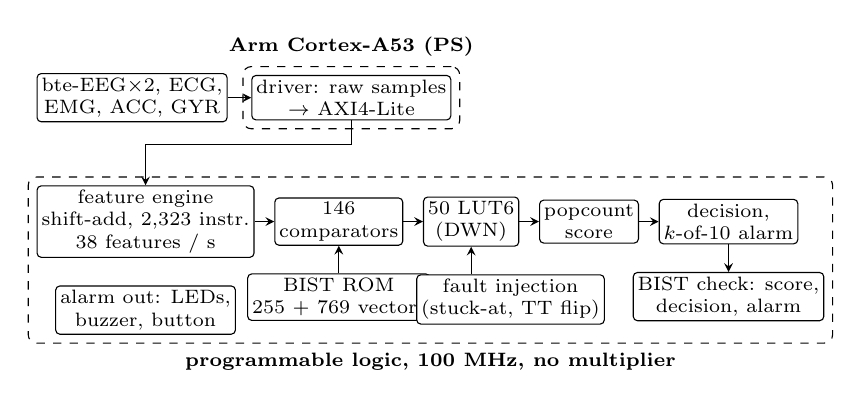
\begin{tikzpicture}[font=\scriptsize, >=stealth,
  blk/.style={draw, rounded corners=1.5pt, align=center, minimum height=5.2mm, inner sep=1.6pt, fill=white},
  grp/.style={draw, dashed, rounded corners=3pt, inner sep=3pt}]
  % Arm side
  \node[blk] (sens) at (0,0) {bte-EEG$\times$2, ECG,\\EMG, ACC, GYR};
  \node[blk, right=3mm of sens] (drv) {driver: raw samples\\$\to$ AXI4-Lite};
  \node[grp, fit=(drv), label={[font=\scriptsize\bfseries]above:Arm Cortex-A53 (PS)}] (ps) {};
  % fabric
  \node[blk, below=8mm of sens.south west, anchor=north west] (fe) {feature engine\\shift-add, 2,323 instr.\\38 features / s};
  \node[blk, right=2.5mm of fe] (cmp) {146\\comparators};
  \node[blk, right=2.5mm of cmp] (lut) {50 LUT6\\(DWN)};
  \node[blk, right=2.5mm of lut] (pop) {popcount\\score};
  \node[blk, right=2.5mm of pop] (alm) {decision,\\$k$-of-10 alarm};
  \node[blk, below=3.5mm of cmp] (rom) {BIST ROM\\255 + 769 vectors};
  \node[blk, below=3.5mm of lut, xshift=5mm] (fi) {fault injection\\(stuck-at, TT flip)};
  \node[blk, below=3.5mm of alm] (chk) {BIST check: score,\\decision, alarm};
  \node[blk, below=3.5mm of fe] (io) {alarm out: LEDs,\\buzzer, button};
  \node[grp, fit=(fe)(alm)(rom)(io)(chk), label={[font=\scriptsize\bfseries]below:programmable logic, 100 MHz, no multiplier}] (pl) {};
  \draw[->] (sens) -- (drv);
  \draw[->] (drv.south) |- ++(0,-3mm) -| (fe.north);
  \draw[->] (fe) -- (cmp);
  \draw[->] (cmp) -- (lut);
  \draw[->] (lut) -- (pop);
  \draw[->] (pop) -- (alm);
  \draw[->] (rom.north) -- (cmp.south);
  \draw[->] (fi.north -| lut.south) -- (lut.south);
  \draw[->] (alm.south) -- (chk.north);
\end{tikzpicture}
}
\caption{SeizeLUT on the Kria KV260. The fault-injection registers and the self-test let the device check that the
fabric still computes the validated classifier.}\label{fig:arch}
\end{figure}

\begin{itemize}
\item \textbf{Interface:} one AXI4-Lite slave at 100\,MHz with an 8-KB window: control and result registers, the
  feature registers, and the feature engine's register file at 0x1000.
\item \textbf{Classifier:} 146 threshold comparators, 50 LUT6, popcount score, frozen and programmable operating
  points, 10-of-10 alarm, latency 3 clock cycles.
\item \textbf{Test logic:} built-in self-test (BIST) with its vector ROM, fault-injection registers, read-back of
  all comparator bits and LUT outputs.
\item \textbf{Demo I/O:} PMOD outputs for an alarm LED, a buzzer, score LEDs and a heartbeat, and a debounced button.
\end{itemize}

\section{Front End in the Fabric}\label{sec:fe-engine}

A front end with dozens of filters would need many multipliers if built directly. Instead, a small microcoded
\emph{feature engine} computes the 38 features the classifier reads, one instruction at a time:

\begin{itemize}
\item one 40-bit adder and two 5-bit shifters; every filter coefficient is a sum of at most five signed powers of
  two, so a multiplication becomes a few shifted additions;
\item a register file (930 words) and a 2,323-instruction program in block RAM, 3 clock cycles per instruction;
\item four events: a 256-Hz biopotential sample, a 25-Hz motion sample, the end of a second, and the last window.
\end{itemize}

After each window the core copies the engine's 38 features into the classifier and classifies them automatically.

\begin{table}[H]
\centering\small
\caption{Verification of the feature engine.}\label{tab:fe-verif}
\begin{tabularx}{\textwidth}{@{}LP{58mm}@{}}
\toprule
\textbf{Check} & \textbf{Result}\\
\midrule
Program (instruction-level simulator) against the C front end, 10 recordings & all 431,960 windows equal (38 features)\\
Engine RTL fed sample by sample (Verilator), EEG-only and all-sensor recording & 4,278 windows, 0 mismatches\\
Whole core from raw samples through AXI (Verilator) & 4,278 windows: features, score, decision, alarm equal\\
On the KV260 board, 3 raw recordings & 9,214 windows, 0 feature and 0 output mismatches\\
Busy cycles per second of signal & at most 946,168 (simulation and board identical)\\
\bottomrule
\end{tabularx}
\end{table}

The engine needs under one million cycles per second of signal, so it keeps up with the sensors at 1\,MHz, a
hundredth of the board's clock.

\section{Hardware Cost}

\begin{table}[H]
\centering\small
\caption{Cost of the LUT-native classifiers on the XCK26 (Vivado 2026.1 out of context, 2.5-ns constraint,
vectorless power at 400\,MHz; Yosys \texttt{synth\_xilinx} as a second flow).}\label{tab:hwcost}
\begin{tabular}{@{}lrrrrrr@{}}
\toprule
\textbf{Model} & \textbf{LUTs} & \textbf{FFs} & \textbf{Fmax} & \textbf{Dyn. power} & \textbf{Yosys LUTs} & \textbf{Test F1}\\
\midrule
\textbf{DWN + distillation (ours)} & \textbf{398} & 454 & \textbf{468\,MHz} & \textbf{17\,mW} & 405 & 0.248\\
TreeLUT (5-bit leaves) & 2,677 & 1,461 & 294\,MHz & 88\,mW & 2,721 & 0.233\\
Logic-gate network & 5,249 & 2,208 & 154\,MHz & 523\,mW & 5,758 & 0.191\\
\bottomrule
\end{tabular}
\end{table}

\begin{table}[H]
\centering\small
\caption{Cost of the whole detector and of the KV260 design (Vivado 2026.1, user's build).}\label{tab:whole}
\begin{tabularx}{\textwidth}{@{}LP{70mm}@{}}
\toprule
\textbf{Part} & \textbf{Cost}\\
\midrule
Feature engine alone (out of context) & 804 LUTs, 101 FFs, 4.5 block RAMs, 0 DSP, 234\,MHz\\
Whole detector (feature engine + DWN) & \textbf{1,202 LUTs, no multiplier} (Yosys: 797 + 405, also 1,202)\\
Whole core in the design (with BIST, fault injection, debug, demo I/O) & 3,356 LUTs, 13.5 block RAMs\\
Full KV260 design & 3,796 LUTs (3.2\,\% of the device), 0 DSP; timing met at 100\,MHz (slack 3.5\,ns)\\
\bottomrule
\end{tabularx}
\end{table}

The DWN needs 6.7 times fewer LUTs than TreeLUT and 13.2 times fewer than the logic-gate network, and it is also the
fastest. Its thermometer comparators, not the network, take most of its cost.

\section{Self-Testing}

\paragraph{Fault model.} Every single fault in the part of the hardware the network adds: each of the $50 \times 64 =
3{,}200$ truth-table bits flipped (an upset in FPGA configuration memory) and each comparator and LUT output stuck at 0
or 1 (292 + 100): 3,592 faults.

\paragraph{Which faults matter.} Each fault was applied to all 31.4 million windows (8,714 hours) of the 96 training
patients. A fault is \emph{decision-relevant} if it changes at least one decision.

\paragraph{Test vectors.} The vectors were chosen from training windows to cover the rarely used truth-table entries
first (Table~\ref{tab:faults}, Figure~\ref{fig:faultcov}).

\begin{table}[H]
\centering\small
\caption{Single faults on the training data and the decision-relevant faults detected (\%) by three self-test vector
sets.}\label{tab:faults}
\begin{tabular}{@{}lrrrrrr@{}}
\toprule
\textbf{Fault} & \textbf{All} & \textbf{Decision} & \textbf{Alarm} & \textbf{Consecutive} & \textbf{Random} &
\textbf{Selected}\\
\midrule
truth-table bit flipped & 3,200 & 2,498 & 1,674 & 43.6 & 79.4 & \textbf{100.0}\\
comparator stuck at 0/1 & 292 & 292 & 289 & 94.5 & 100.0 & \textbf{100.0}\\
LUT output stuck at 0/1 & 100 & 100 & 100 & 100.0 & 100.0 & \textbf{100.0}\\
\midrule
\textbf{all} & 3,592 & 2,890 & 2,063 & 50.7 & 82.2 & \textbf{100.0}\\
\bottomrule
\end{tabular}
\end{table}

\begin{figure}[H]
\centering
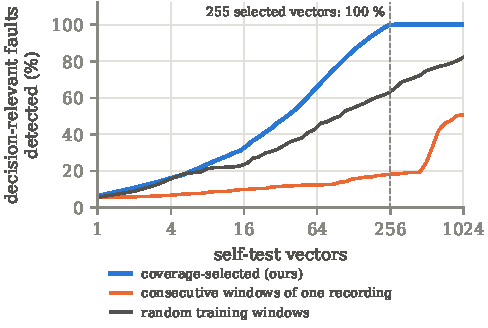
\includegraphics[width=0.75\textwidth]{figures/fault_coverage.pdf}
\caption{Decision-relevant faults detected by the first $m$ self-test vectors.}\label{fig:faultcov}
\end{figure}

The natural choice of a test, 1,024 consecutive recorded windows, detects only 50.7\,\% of the faults that change a
decision; the 255 selected windows detect all of them. The on-chip self-test runs 1,024 vectors in 1,028 clock cycles
(10.3\,\textmu s), so the device can test itself after every one-second window.

\section{Board Results}

The board runs Ubuntu 22.04 with Kria-PYNQ. One script (\texttt{run\_board\_tests.sh}) runs nine tests and saves all
numbers to a results file. Table~\ref{tab:board} gives the full campaign on our KV260.

\begin{table}[H]
\centering\small
\caption{Board test campaign on the KV260 (kit v6 bitstream, Vivado 2026.1).}\label{tab:board}
\begin{tabularx}{\textwidth}{@{}P{38mm}LP{22mm}@{}}
\toprule
\textbf{Step} & \textbf{Measured on the board} & \textbf{Result}\\
\midrule
1 Identity & core version 3, 38 features, 50 LUTs; bitstream loads in 4.4\,s & PASS\\
2 Self-test & 1,024 of 1,024 vectors correct in 1,028 cycles & PASS\\
3 Latency & 3 clock cycles (30\,ns) & PASS\\
4 Replay & all 431,960 windows of 10 recordings through the registers: 0 mismatches at both operating points;
  3.2\,\textmu s per window & PASS\\
5 Detection (10 recordings) & frozen point: 1 of 19 seizures, 0 false alarms in 120\,h; programmable point: 3 of 19,
  25 false alarms (equal to simulation) & reported\\
6 Power & 3.069\,W idle, 3.074\,W with the classifier fed one window per clock (difference within the sensor's
  noise) & reported\\
7 Front end on the Arm & 3 raw recordings: 0 feature and 0 output mismatches, 3,390--4,080 times faster than real
  time & PASS\\
8 Fault injection & all 3,592 faults injected: 0 hardware/software mismatches; all 2,890 decision-relevant faults
  detected; 88\,s & PASS\\
9 Whole detector in the fabric & 9,214 windows from raw samples: 0 feature and 0 output mismatches; engine busy
  for exactly the simulated cycles (787,615 / 787,521 / 946,168 per second); 102--124 times faster than real time &
  PASS\\
\bottomrule
\end{tabularx}
\end{table}

Step 5 covers only the 10 exported recordings of three test patients, as a check that the board reproduces the
software; the detection results on all 29 test patients are in Chapter~\ref{ch:results}. The first board run found one
software bug: the driver wrote ``soft reset'' and ``clear counters'' in the same register write, and the hardware
gives the reset priority, so the counters were not cleared. The driver now writes them separately (no rebuild).

\section{Live Demo}

Recorded test-patient signals stream second by second through the board, and a laptop browser shows every stage:
signals, features, comparator bits, LUT votes, score and alarm, with a check on every window that the FPGA equals the
software (Figure~\ref{fig:dashboard}). On the breadboard, the FPGA drives a red alarm LED (PMOD B1, 220\,$\Omega$) and
a buzzer through a BC547 transistor (PMOD B2, 1\,k$\Omega$). On the board the alarm fires during the seizure and the
LED and buzzer turn on.

\begin{figure}[H]
\centering
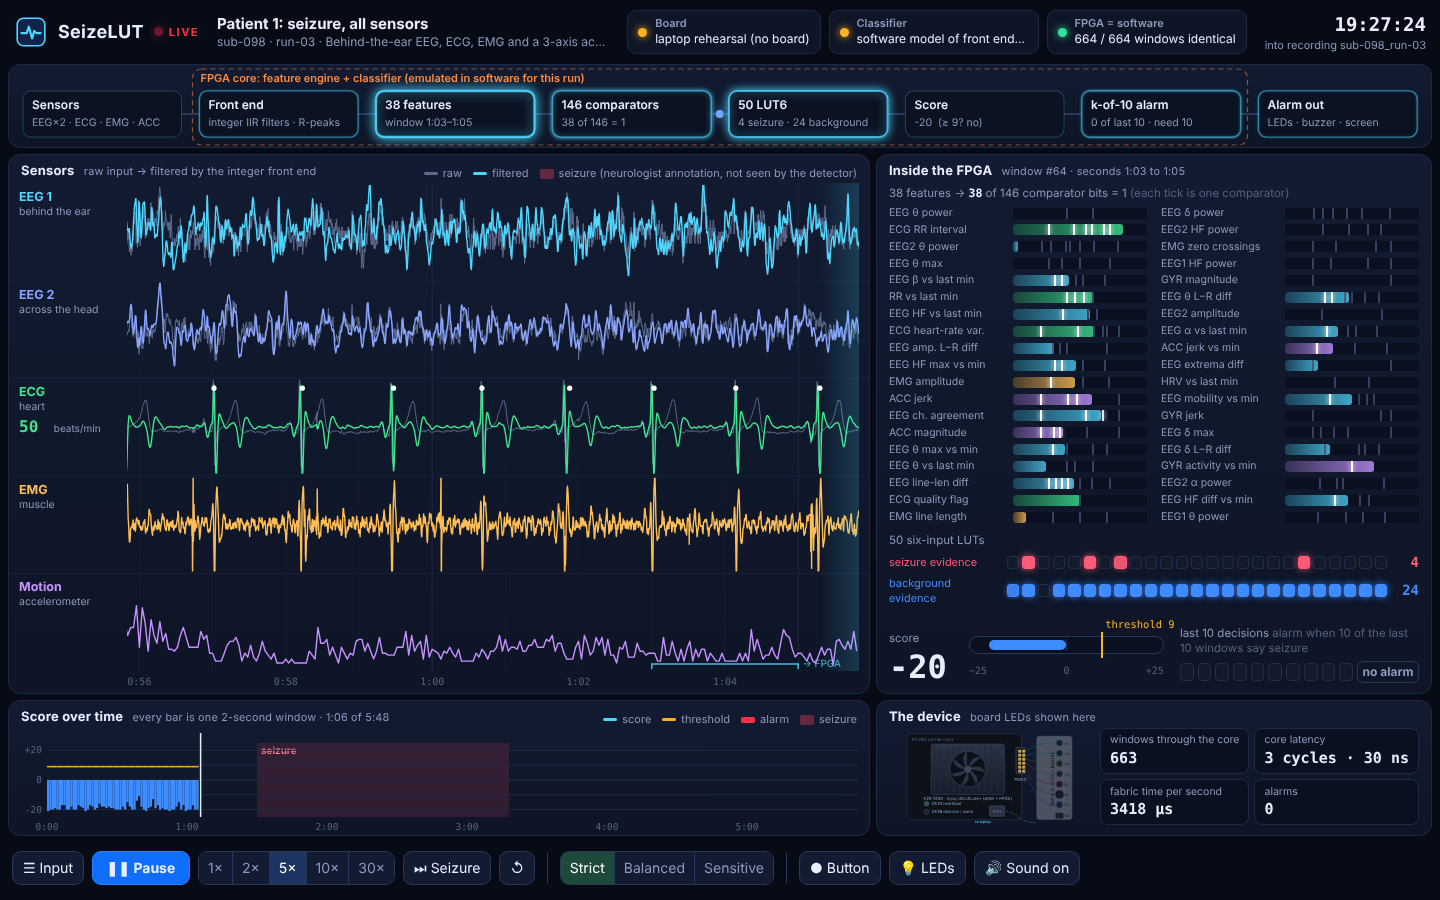
\includegraphics[width=\textwidth]{figures/dashboard_rehearsal.png}
\caption{Live dashboard (laptop rehearsal with the software model of the core; on the board the same page shows the
FPGA).}\label{fig:dashboard}
\end{figure}

\chapter{Doctor Alert with an ESP32}\label{ch:alert}

An alarm helps only if someone can act on it quickly. When the KV260 raises an alarm, an ESP32 on the same breadboard
tells the doctor, who may be in a cabin or another room.

\section{Architecture}

\begin{itemize}
\item \textbf{Board to ESP32:} the board sends one short message per event over the ESP32's USB cable (alarm start,
  updates every 15\,s, escalations, end, patient button). The FPGA's alarm pin (PMOD B1) is also wired to an ESP32
  input as a backup that works even if the board's software stops. The USB cable also powers the ESP32.
\item \textbf{ESP32 to phone:} the ESP32 joins the phone's Wi-Fi hotspot and sends a push notification through the
  ntfy service (iPhone and Android app), and serves a live alarm page on the same network.
\item \textbf{Phone to board:} the doctor's ``On my way'' reaches the ESP32 and is sent back to the board, where the
  dashboard shows it.
\end{itemize}

\section{What the Doctor Sees}

The detector answers ``seizure-like or not''; it was not trained to name a seizure type, so the alert reports only
signs that the front end measures, compared with the minute before the alarm:

\begin{table}[H]
\centering\small
\caption{The signs in the alert.}\label{tab:signs}
\begin{tabularx}{\textwidth}{@{}lLP{50mm}@{}}
\toprule
\textbf{Sign} & \textbf{Shown as} & \textbf{Measured from}\\
\midrule
Heart rate & before and now, NORMAL / HIGH / VERY HIGH & ECG R-peak intervals\\
Shaking & LITTLE / SOME / STRONG & chest accelerometer (or gyroscope)\\
Muscle tension & NORMAL / HIGH & EMG power\\
Brain activity & MILD / HIGH, slow or fast waves & EEG line length and band power\\
Pattern hint & ``motor pattern likely'' or ``little movement'' & movement change\\
\bottomrule
\end{tabularx}
\end{table}

Because the doctor has very little time, the alert is made to be read in about two seconds:

\begin{itemize}
\item \textbf{Notification:} three lines, for example ``SEIZURE Bed 3 / GO TO BED 3 NOW: PROTECT FROM INJURY / Heart
  120 bpm HIGH \textbar{} Shaking STRONG \textbar{} Brain HIGH''.
\item \textbf{Page (Figure~\ref{fig:alertpage}):} status and a running timer; one instruction; ``On my way'' and
  ``Call'' buttons; four colour tiles (red = act, amber = watch, green = normal). The patient's emergency plan, first-aid
  steps and exact numbers are folded below.
\item \textbf{One instruction}, the most urgent first: CHECK BREATHING AND PULSE NOW (heart rate above 150 or below
  40\,bpm, or an unreadable ECG without shaking) $>$ OVER 5 MIN: START EMERGENCY PLAN $>$ OVER 2 MIN: GET EMERGENCY
  PLAN READY $>$ GO TO BED NOW: PROTECT FROM INJURY (strong shaking) $>$ GO TO BED NOW. When it ends: SEIZURE STOPPED:
  CHECK BREATHING, TURN ON SIDE.
\item \textbf{Escalation} at 2 and 5 minutes of alarm, then every minute. Five minutes is the ILAE time point for
  treating a convulsive seizure as status epilepticus; the seizure starts before the alarm, so the real duration is
  longer.
\item \textbf{Reminders} every minute until someone taps ``On my way''; \textbf{clusters} (``2nd seizure this
  hour'') are flagged; no patient names are sent, only a bed name.
\end{itemize}

\begin{figure}[H]
\centering
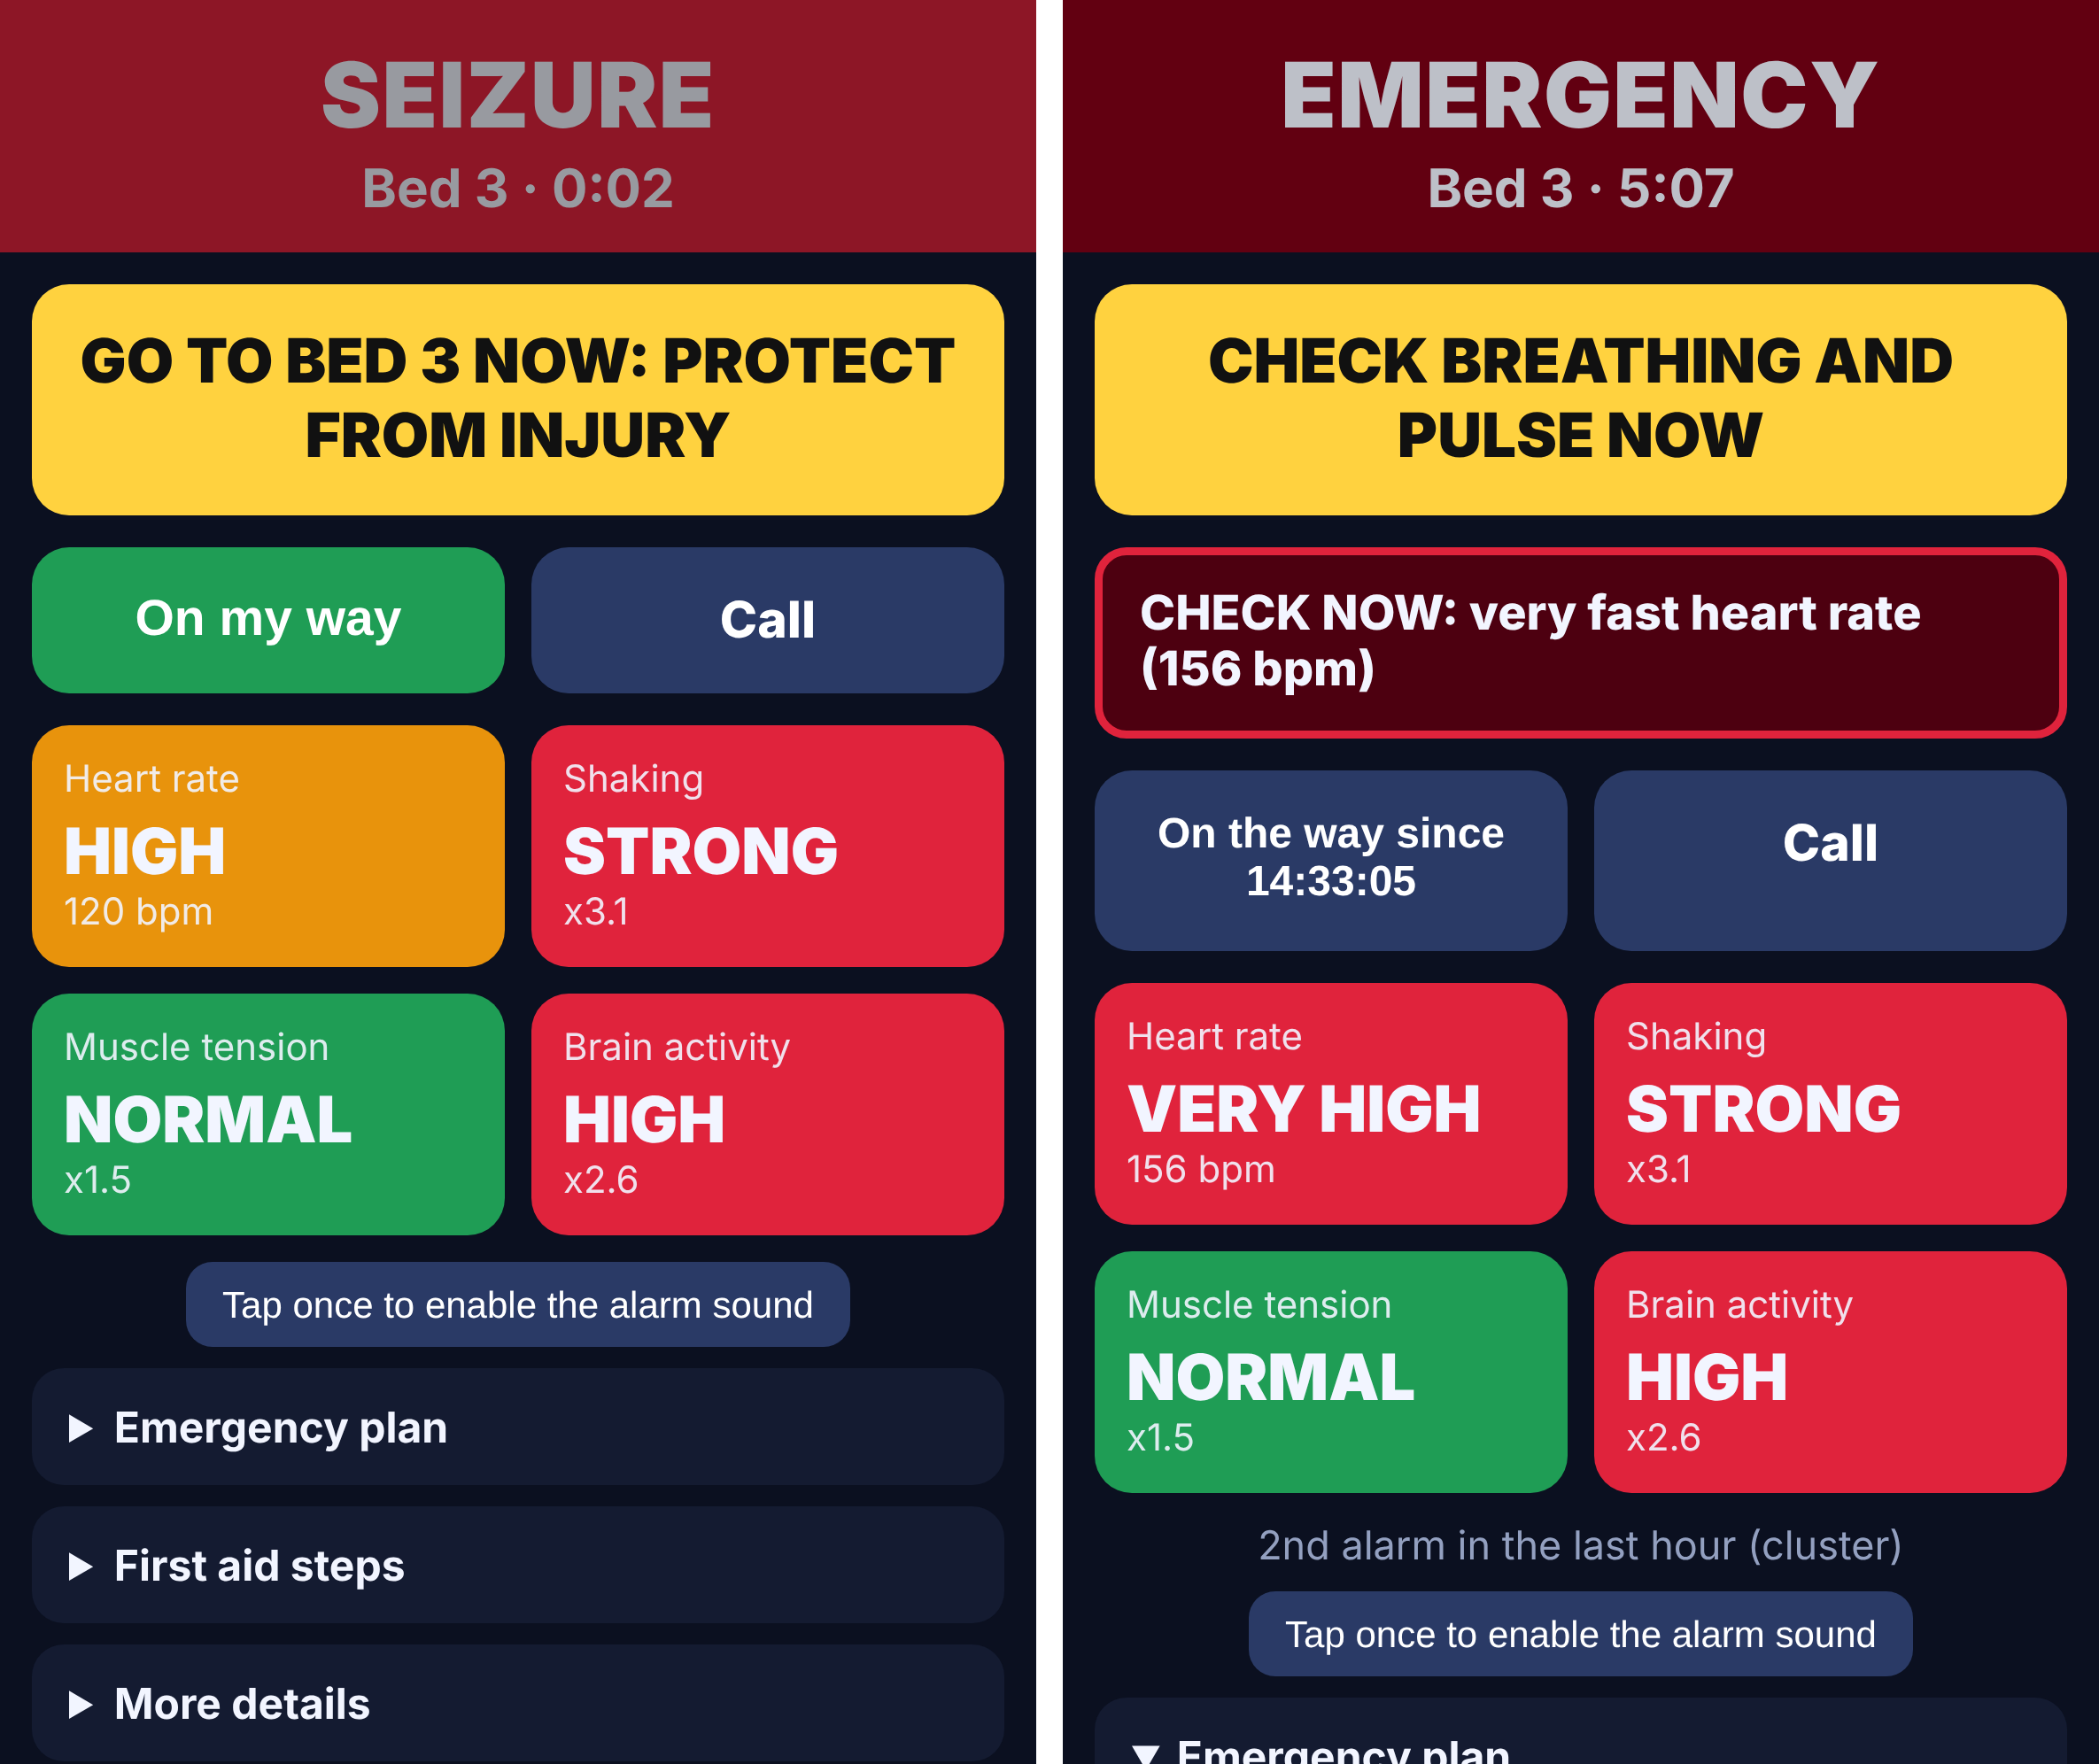
\includegraphics[width=0.9\textwidth]{figures/alert_page.png}
\caption{The doctor's page at a new seizure (left) and in an emergency after 5 minutes (right).}\label{fig:alertpage}
\end{figure}

\section{How Good Is the Pattern Hint?}

We checked the movement-based hint against the doctors' motor / non-motor labels of the 702 seizures of the training
patients only (the test patients were not read):

\begin{itemize}
\item In the first 30\,s, movement rose 4.8-fold (median) in motor seizures and 1.04-fold in non-motor seizures;
  heart rate rose 17\,\% and 8\,\%.
\item A threshold (2.6-fold) chosen on patients 1--48 matched the doctors' label on patients 49--96 in 64\,\% of
  cases (balanced accuracy: 48\,\% of motor and 79\,\% of non-motor seizures). Adding EMG did not help.
\item So the hint is useful but not a diagnosis. The two EEG inputs are one behind-the-ear and one cross-head
  channel chosen per recording, so the alert makes no left/right claim.
\end{itemize}

\section{Testing}

The board side was tested on the emulated board through a virtual serial port: alarm start, updates, end after 30\,s
of quiet, escalation at 2, 5, 6 and 7 minutes (none after the alarm stops), clusters, and the acknowledgement coming
back. The ESP32 program passes a syntax check and the page was rendered at iPhone size. The test on the ESP32 itself,
with a real iPhone, is the next step.

\chapter{Challenges Faced and How They Were Addressed}\label{ch:challenges}

\begin{xltabular}{\textwidth}{@{}P{17mm}P{40mm}LL@{}}
\caption{The main problems and their solutions.}\label{tab:challenges}\\
\toprule
\textbf{Area} & \textbf{Challenge} & \textbf{What happened} & \textbf{Solution}\\
\midrule
\endfirsthead
\toprule
\textbf{Area} & \textbf{Challenge} & \textbf{What happened} & \textbf{Solution}\\
\midrule
\endhead
\bottomrule
\endlastfoot
\small Data & \small Files differ from the documentation & \small 256 Hz not 250 Hz; 883 not 886 seizures; no centre
or age labels & \small Full audit first; design follows the files\\
\small Data & \small 126 GB, no local disk or GPU & \small Dataset too large for the server & \small Stream, extract,
delete: only 3.5 GB of features kept\\
\small Data & \small Silent download truncation & \small 9 recordings cut short (one EEG file: 12 of 16,363 windows) &
\small Size checks; re-extracted; 3 runs repeated\\
\small Data & \small Official artefact rule & \small Flags 69\,\% of normal behind-the-ear windows & \small Flags used
as input bits; gating chosen on training folds\\
\small Baseline & \small ChronoNet only partly reproduced & \small 74.5\,\% vs 84.2\,\% detected & \small Literal port
(identical on 900 test cases); gap reported as measured\\
\small Baseline & \small Released code tunes on the test patients & \small Best epoch picked on the evaluation
patients & \small Clean run with no test information as our reference\\
\small Baseline & \small SVM features unavailable & \small Defined in a paper we could not access & \small Open;
requested for Phase II\\
\small Hardware & \small Rounding noise in integer filters & \small Error 140 LSB, larger than the signal (61 LSB) &
\small Error feedback: 0.7 LSB\\
\small Hardware & \small Heart rate needs a division & \small $60/\mathrm{RR}$ & \small $\log_2(\mathrm{RR})$: no
division or multiplication\\
\small Hardware & \small Verilog disagreed with software & \small Thresholds beyond a feature's bit width & \small
Generator fixed: 0 mismatches\\
\small Compute & \small 6 GB laptop GPU; CUDA-only library & \small DWN could not run on the CPU server & \small
PyTorch re-implementation, unit-tested against the kernel\\
\small Compute & \small Interrupted runs; out of memory & \small Lost folds; a sampler used 13.9 GB & \small Resumable
runs; new sampler peaks at 3.1 GB\\
\small ML & \small Seizures are 0.123\,\% of the time & \small Accuracy is meaningless & \small Event scoring per
patient; balanced sampling; false-alarm budget\\
\small ML & \small \textbf{Weak early results} & \small First network: event-F1 0.148, 7.0 false alarms/day & \small
N7 showed heart rate was ignored; new feature selection: 0.208, 2.3/day\\
\small ML & \small Bugs in comparisons & \small Wrong feature set; distillation lost on retraining & \small Found in
run records; shared training code, tests, runs repeated\\
\small FPGA & \small Front end needs many multipliers & \small Dozens of filters per window & \small Microcoded
shift-add engine: 804 LUTs, no DSP\\
\small FPGA & \small Engine and bus raced each other & \small For one clock cycle the core reported idle before the
feature transfer, writes were lost & \small Found by the end-to-end testbench before the build; idle condition fixed\\
\small Board & \small Counters not cleared on the board & \small Reset and clear in one write; the emulator hid it &
\small Two separate writes; emulator now copies the hardware\\
\small Board & \small No network for the board & \small Board has no Wi-Fi; phone hotspot only & \small Kit copied with
a USB drive; tests need no network\\
\small Demo & \small LED always on, buzzer silent & \small Wires on the wrong end of the PMOD connector; buzzer (+) not
on 3.3\,V & \small Pin test script; wiring table in the guide\\
\small Alert & \small Too much information for a doctor in a hurry & \small Long text with numbers & \small One
instruction, four colour tiles, three-line notification\\
\small Alert & \small False ``check breathing'' during shaking & \small Shaking spoils the ECG & \small ECG flag only
without shaking\\
\end{xltabular}

\chapter{Conclusions, Publication Plan and Future Work}\label{ch:concl}

\section{Conclusions}

\begin{itemize}
\item \textbf{A complete multiplier-free detector:} a 50-LUT weightless network on integer multimodal features
  reaches an event-F1 of 0.248 with 0.8 false alarms per day on 29 held-out patients; with its front end in the
  fabric the whole detector needs 1,202 LUTs and no multiplier.
\item \textbf{Accuracy per LUT:} above TreeLUT at a seventh of its LUTs, above the logic-gate network, the INT8 network
  and ChronoNet; level with random forest and CatBoost; below LightGBM, which needs about 30,000 LUTs.
\item \textbf{Above the dataset paper's SVM} at its false-alarm rate with post-ictal verification (73.3\,\% against
  71.1\,\% of seizures).
\item \textbf{Self-testing:} all 3,592 single faults analysed; 255 selected vectors detect every fault that changes a
  decision; confirmed fault by fault on the board.
\item \textbf{Working hardware:} all nine board tests pass on the KV260; the cycle counts on the board equal the
  simulation exactly; the live demo drives an alarm LED and a buzzer.
\item \textbf{Doctor alert:} a phone notification that says what to do, with escalation and acknowledgement.
\item \textbf{Limits:} focal seizures are still mostly missed, as in the clinical literature
  \cite{beniczky2021guideline}; results come from retrospective recordings of one dataset; the ESP32 alert still has to
  be tested on the ESP32 itself.
\end{itemize}

\section{Publication Plan}

A 6-page paper with all results, including the board measurements, is ready. The best-fitting venues and their
deadlines (official conference pages, checked on 20 November 2026):

\begin{table}[H]
\centering\small
\caption{Candidate conferences.}\label{tab:venues}
\begin{tabularx}{\textwidth}{@{}lP{38mm}L@{}}
\toprule
\textbf{Conference} & \textbf{Deadline} & \textbf{Fit}\\
\midrule
IEEE EMBC 2027 & full paper 24 Jan 2027 & biomedical engineering; new limit of 4 pages + 1 page of references, so the paper must
  be shortened\\
IEEE/ACM FCCM 2027 & abstract 10 Jan, paper 17 Jan 2027 & FPGA hardware: the self-testing and the fabric front end\\
IEEE BioCAS 2027 & abstract 7 May 2027 (Oslo, 14--16 Oct 2027) & biomedical circuits and systems: the best overall fit
  for the whole system\\
\bottomrule
\end{tabularx}
\end{table}

\section{Future Work}

\begin{itemize}
\item Test the doctor alert on the ESP32 with a real phone; measure the time from seizure alarm to notification.
\item Detect more focal seizures, the main clinical gap.
\item Prospective recordings with the board worn by volunteers, and a battery-powered low-power FPGA.
\item Run the self-test periodically in the field and react to a failed test.
\end{itemize}


% ================================================================ references and appendices
\cleardoublepage
\phantomsection
\addcontentsline{toc}{chapter}{References}
\renewcommand{\bibname}{References}
\markboth{References}{}
{\small\singlespacing
\bibliographystyle{IEEEtran}
\bibliography{refs}}

\appendix
\chapter{Full Results and Sources}\label{app:sources}

\section{All Models on the 29 Test Patients}

\begin{table}[htbp]
\centering\footnotesize
\caption[Final evaluation of every model on the 29 test patients.]{Final evaluation of every model on the 29 test patients (5 seeds; SzCORE event metrics at the best-F1
operating point chosen on the training folds; Paper: the base paper's sensitivity and false alarms per hour; $p$: paired
Wilcoxon on per-patient event-F1).}\label{tab:test-full}
\setlength{\tabcolsep}{2pt}
\begin{tabular}{@{}lcccccccc@{}}
\toprule
\textbf{Model} & \textbf{AUROC} & \textbf{Event-F1} & \textbf{Sens} & \textbf{Prec} & \textbf{FA/24\,h} &
\textbf{Paper} & \textbf{Cost} & \textbf{$p$ vs LGBM}\\
\midrule
\textbf{DWN + distillation (final)} & 0.883 & \textbf{0.248} & 0.303 & 0.291 & 0.8 & 25.5\,\% / 0.02 & 895 LUTs & 0.039\\
DWN + modality dropout & 0.866 & 0.242 & 0.272 & 0.282 & 0.4 & 21.7\,\% / 0.01 & 951 LUTs & 0.035\\
DWN base & 0.875 & 0.172 & 0.340 & 0.156 & 2.7 & 29.2\,\% / 0.12 & 980 LUTs & 0.004\\
LightGBM & 0.877 & 0.308 & 0.331 & 0.396 & 0.6 & 26.8\,\% / 0.01 & 30,750 LUTs & --\\
XGBoost & 0.872 & 0.294 & 0.301 & 0.387 & 0.4 & 25.1\,\% / 0.01 & 48,295 LUTs & 0.29\\
CatBoost & 0.874 & 0.254 & 0.330 & 0.281 & 1.2 & 25.8\,\% / 0.04 & 27,720 LUTs & 0.026\\
Random forest & 0.858 & 0.246 & 0.245 & 0.305 & 0.2 & 22.4\,\% / 0.00 & 346,576 LUTs & 0.35\\
TreeLUT (5-bit leaves) & 0.858 & 0.233 & 0.292 & 0.296 & 1.0 & 25.1\,\% / 0.04 & 6,330 LUTs & 0.005\\
Logic-gate network & 0.865 & 0.191 & 0.291 & 0.186 & 1.4 & 23.1\,\% / 0.06 & 7,452 LUTs & 0.008\\
INT8 MLP & 0.788 & 0.155 & 0.249 & 0.163 & 1.7 & 21.8\,\% / 0.10 & 9,600 mult. & 0.005\\
Logistic regression & 0.814 & 0.123 & 0.255 & 0.096 & 5.1 & 23.0\,\% / 0.27 & 117 mult. & 0.0008\\
ChronoNet (clean, 1 seed) & -- & 0.027 & 0.790 & 0.015 & 106.3 & 67.1\,\% / 11.9 & CNN + GRU & --\\
\bottomrule
\end{tabular}
\end{table}

\section{Sources of the Reported Numbers}

Every number in this report comes from a saved result file; each run folder holds the configuration, code version,
log and metrics.

\begin{xltabular}{\textwidth}{@{}P{62mm}L@{}}
\caption{Sources of the reported numbers.}\label{tab:sources}\\
\toprule
\textbf{Numbers} & \textbf{Source}\\
\midrule
\endfirsthead
\toprule
\textbf{Numbers} & \textbf{Source}\\
\midrule
\endhead
\bottomrule
\endlastfoot
\small Dataset inventory and audit (Chapter~\ref{ch:method}) & \small \texttt{reports/data\_audit.md},
\texttt{results/audit/}\\
\small Fixed-point specification & \small \texttt{spec/fixed\_point.md}\\
\small Integer vs floating point (Table~\ref{tab:intfloat}) & \small \texttt{results/m3/int\_float\_gap.md}\\
\small ChronoNet reproduction (Figure~\ref{fig:chrononet}) & \small runs \texttt{20261107-125159\_chrononet\_official\_s1},
\texttt{20261107-204035\_chrononet\_clean\_s1}\\
\small Model families (Table~\ref{tab:families}) & \small \texttt{results/tables/inner\_cv.md}\\
\small Extensions, missing sensors (Figures~\ref{fig:ablation},~\ref{fig:missing}) & \small
\texttt{results/tables/m5\_ablation.md}; \texttt{breakdown.json} in each run folder\\
\small Final test (Tables~\ref{tab:test},~\ref{tab:test-full}) & \small \texttt{results/tables/final\_test.md}\\
\small Base-paper comparison (Figure~\ref{fig:sensfa}) & \small \texttt{results/tables/sens\_fa\_test.json}\\
\small Verilog check (Table~\ref{tab:verilog}) & \small \texttt{export/n4\_distill\_s0/verilog\_check.json}\\
\small Decisions and their evidence & \small \texttt{results/decisions.md}\\
\end{xltabular}


\end{document}
